\documentclass[a4paper,12pt]{report}

% Page layout
\usepackage[left=2.5cm,right=2.5cm,top=2.5cm,bottom=2.5cm]{geometry}

% Font and text
\usepackage[british,afrikaans]{babel}
\usepackage{microtype}
\usepackage{setspace}
\usepackage{lmodern}
\usepackage{siunitx}
\newcommand{\myemph}[1]{{\sffamily\bfseries#1}}
\sloppy
\onehalfspacing

% Headings
\usepackage[raggedright,sf,bf]{titlesec}
\usepackage[margin=\the\parindent,small,bf,sf]{caption}
\titlelabel{\thetitle.\ }
\titleformat{\chapter}[display]{\huge\bfseries\sffamily}{\chaptertitlename\ \thechapter}{15pt}{\Huge \raggedright}
\titlespacing*{\chapter}{0pt}{0pt}{40pt}  % remove spacing before chapter headings
\makeatletter
\let\originall@chapter\l@chapter
\def\l@chapter#1#2{\originall@chapter{{\sffamily #1}}{#2}}
\makeatother

%% Alternative headings using small-caps (comment out the top section)
%\usepackage[raggedright,bf]{titlesec}
%\usepackage[margin=\the\parindent,small,bf]{caption}
%\titlelabel{\thetitle.\ }
%\titleformat{\chapter}[display]{\huge\scshape}{\chaptertitlename\ \thechapter}{15pt}{\Huge \raggedright}
%\titlespacing*{\chapter}{0pt}{0pt}{40pt}  % remove spacing before chapter headings

% Table of contents
\let \savenumberline \numberline
\def \numberline#1{\savenumberline{#1.}}

% Figures
\usepackage{graphicx} % JPG, PNG, PDF images
\usepackage{svg} % SVG images
\usepackage{pdfpages}
\usepackage{float}
\usepackage{subcaption}
\setlength{\abovecaptionskip}{7.5pt}  % spacing above and below captions
\newcommand*{\WaterMark}[2][0.2\paperwidth]{\AddToShipoutPicture*{\AtTextCenter{\parbox[c]{0pt}{\makebox[0pt][c]{\includegraphics[width=#1]{#2}}}}}}

% TikZ
\usepackage{tikz}
\usetikzlibrary{shapes, shadows, arrows, arrows.meta}
\usetikzlibrary{fit}
\usetikzlibrary{external}
\tikzexternalize % activate!

% Plots
\usepackage{pgfplots} % plots
\pgfplotsset{width=\columnwidth, compat=newest} % plot parameters
\usepgfplotslibrary{units} % allows to enter the units nicely
\usepgfplotslibrary{colorbrewer} % awesome colors

% Color
\usepackage{xcolor}
\definecolor{light_blue}{RGB}{222,235,247}
\definecolor{faded_red}{RGB}{203,24,29} % #CB181D

% Mathematics
\usepackage[cmex10]{amsmath}
\usepackage{mathtools}
\usepackage{bm}
\usepackage{amssymb}
\usepackage{cancel}
\usepackage{siunitx} % SI Units
\usepackage{tabstackengine}
\newcolumntype{M}[1]{>{\centering\arraybackslash$}m{#1}<{$}} % Middle (don't clash with C from tabularx)
\newlength{\mycolwd} % array column width
\settowidth{\mycolwd}{$\bm{x}_{w+q-1}$} % "width" of largest element in array
\stackMath
\DeclareMathOperator*{\argmax}{arg\,max}
\newcommand{\T}{^\top}
\newcommand{\tr}{\textrm{tr}}
\renewcommand{\vec}[1]{\boldsymbol{\mathbf{#1}}}
\newcommand{\defeq}{\triangleq}
\newcommand{\R}{\mathbb{R}}

% Tables
\usepackage{booktabs}
\usepackage{tabularx}
\usepackage{multirow}
\newcommand{\mytable}{
    \centering
    \small
    \renewcommand{\arraystretch}{1.2}
    }
\renewcommand{\tabularxcolumn}[1]{m{#1}}
\newcolumntype{C}{>{\centering\arraybackslash}X}
\newcolumntype{L}{>{\raggedright\arraybackslash}X}

% Header and footer
\usepackage{fancyhdr}
\pagestyle{fancy}
\fancyhf{}
\renewcommand{\sectionmark}[1]{\markright{\normalsize \thesection.\ #1}}
\fancyhead[C]{\nouppercase{\textit{\rightmark}}}
\fancyhead[RO]{\thepage}
%\fancyhead[LE]{\thepage}  % double-sided printing
\fancyfoot{}
\setlength\headheight{14.5pt}
\renewcommand{\headrulewidth}{0pt}
\fancypagestyle{plain}{\fancyhead{}
                       \renewcommand{\headrulewidth}{0pt}
                       \fancyfoot[C]{\thepage}}

% Pseudo-code
\usepackage{algorithm}  % should go before \usepackage{hyperref}

% Table of contents and hyperlinks
\usepackage{hyperref}
\hypersetup{colorlinks=true,linktoc=all,citecolor=black,linkcolor=black}
\usepackage[nottoc]{tocbibind}

% Pseudo-code
\usepackage{algpseudocode}  % should go after \usepackage{hyperref}
\renewcommand{\thealgorithm}{\arabic{chapter}.\arabic{algorithm}} 
\captionsetup[algorithm]{labelfont={bf,sf},font=small,labelsep=colon}

% Bibliography
\usepackage{cite}  % automatically reorder inline citations
\bibliographystyle{IEEEtran}
% \usepackage[hyphens]{url}

% Fix titlesec issue
\usepackage{etoolbox}
\makeatletter
\patchcmd{\ttlh@hang}{\parindent\z@}{\parindent\z@\leavevmode}{}{}
\patchcmd{\ttlh@hang}{\noindent}{}{}{}
\makeatother

% Itemize modifications
\usepackage{enumitem}

% Editing
\usepackage{xcolor}
\newcommand{\murray}[1]{\textcolor{blue}{#1}}
\newcommand{\willem}[1]{\textcolor{red}{#1}}

% Glossary
% \usepackage[acronym, nomain, nopostdot, nonumberlist, nogroupskip, toc, automake=false]{glossaries}
%\loadglsentries{glossary}

%%%%%%%%%%%%%%%%%%%%%%%%%%%%%%%%%%%%%%%%%%%%%%%%%%%%%%%%%%%%%%%%%%%%%%%%
\begin{document}

% Front matter
\graphicspath{{frontmatter/fig/}}
\pagenumbering{Alph}

\begin{titlepage}
	\begin{center}
		
		%
\includegraphics[width=10cm]{USlogo-top}
		
		\WaterMark{UScrest-WM}
		
		~\vspace{4.5em}
		
		{\sffamily \bfseries \huge Data-Driven System Identification etc \par}
%		{\scshape \huge A Critical Analysis of Design Flaws in the Death Star \par}		
		
		\vspace{7em}
		
		{\large {\Large  Luke Skywalker} \\ 99652154 \par}
		
		\vspace{8em}
		
		{\large Thesis presented in partial fulfilment of the requirements for the degree of \\ Master of Engineering (Electronic) in the Faculty of Engineering at Stellenbosch University. \par}
		
		\vfill
		
		{\large {Supervisor}: Dr O.\ W.\ Kenobi\\
		Department of Electrical and Electronic Engineering \par}
		
		%\vfill
		\vspace{10em}
		
		{\Large October 2099}
	\end{center}
\end{titlepage}

\pagenumbering{roman}
\chapter*{Acknowledgements}
% \addcontentsline{toc}{chapter}{Acknowledgements}
\makeatletter\@mkboth{}{Acknowledgements}\makeatother

\paragraph
I am ever so grateful for the following people who have had a great influence on this work and on my life:
\begin{itemize}
    \item Dr Willem Jordaan, for his encouragement, guidance, and great conversations.
    \item My family, Arno, Anr\'e, Est\`e and Retief Louw, for their steadfast love.
    \item Chelaine Maree, for her unwavering support and joyful companionship in a challenging year.
    \item My colleagues in the ESL, for helping hands and great times of fun.
\end{itemize}
%\chapter*{Declaration}
\newpage
\thispagestyle{plain}
\addcontentsline{toc}{chapter}{Declaration}
\makeatletter\@mkboth{}{Declaration}\makeatother

\centerline{
\includegraphics[width=8cm]{USlogo-top}}
\vspace*{-10pt}

\section*{\centering Plagiaatverklaring / \textit{Plagiarism Declaration}}

\vspace*{5pt}

\begin{enumerate}
    \item Plagiaat is die oorneem en gebruik van die idees, materiaal en ander intellektuele eiendom van ander persone asof dit jou eie werk is.\\
    \textit{Plagiarism is the use of ideas, material and other intellectual property of another's work
        and to present is as my own.}
    
    \item Ek erken dat die pleeg van plagiaat 'n strafbare oortreding is aangesien dit 'n vorm van diefstal is.\\
    \textit{I agree that plagiarism is a punishable offence because it constitutes theft.}
    
    \item Ek verstaan ook dat direkte vertalings plagiaat is. \\
    \textit{I also understand that direct translations are plagiarism.}
    
    \item Dienooreenkomstig is alle aanhalings en bydraes vanuit enige bron (ingesluit die internet) volledig verwys (erken). Ek erken dat die woordelikse aanhaal van teks sonder aanhalingstekens (selfs al word die bron volledig erken) plagiaat is. \\
    \textit{Accordingly all quotations and contributions from any source whatsoever (including the internet) have been cited fully. I understand that the reproduction of text without quotation marks (even when the source is cited) is plagiarism}
    
    \item Ek verklaar dat die werk in hierdie skryfstuk vervat, behalwe waar anders aangedui, my eie oorspronklike werk is en dat ek dit nie vantevore in die geheel of gedeeltelik ingehandig het vir bepunting in hierdie module/werkstuk of 'n ander module/werkstuk~nie. \\
    \textit{I declare that the work contained in this assignment, except where otherwise stated, is my original work and that I have not previously (in its entirety or in part) submitted it for grading in this module/assignment or another module/assignment.}
\end{enumerate}

\vfill

\noindent \begin{tabularx}{1.0\linewidth}{|L|L|}
    \hline
    \vspace{1cm} {Studentenommer / \textit{Student number}} & \vspace{1cm} {Handtekening / \textit{Signature}} \\
    \hline
    \vspace{1cm} {Voorletters en van / \textit{Initials and surname}} & \vspace{1cm} {Datum / \textit{Date}} \\
    \hline
\end{tabularx}

\vspace{15pt}

% The old declaration

%I, the undersigned, hereby declare that the work contained in this report is my own original work unless otherwise stated.
%
%% Afrikaans:
%% Hiermee verklaar ek, die ondergetekende, dat die werk in hierdie verslag vervat my eie oorspronklike werk is, tensy anders vermeld.
%
%\vspace{2.5cm}
%
%\begin{table}[h]
%\begin{tabular}{@{}p{2.5cm}p{5cm}}
%    Signature: & \dotfill \\
%    & \multicolumn{1}{c}{Obi-Wan Kenobi} \\
%    ~\vspace{1cm} \\
%    Date: & \dotfill \\
%\end{tabular}
%\end{table}
%
%\vfill
%
%\begin{center}
%    Copyright \textcopyright\ 2099 Stellenbosch University \\
%    All rights reserved
%\end{center}


\chapter*{Abstract}
\addcontentsline{toc}{chapter}{Abstract}
\makeatletter\@mkboth{}{Abstract}\makeatother

\vspace{-5mm}
\paragraph
This thesis considers the problem of stabilised control for a multirotor with an unknown suspended payload.
The swinging payload negatively affects the multirotor flight dynamics by inducing oscillations in the system.
An adaptive control architecture is proposed to damp these oscillations and produce stable flight with different unknown payloads.
The architecture includes a data-driven system identification method that assumes no prior knowledge of the payload dynamics.
This method is demonstrated in simulation and with practical flight data.
\gls{MPC} is applied for swing damping control and is verified with \gls{HITL} simulations.  

\paragraph
A parameter estimator and \gls{LQR} is used as a baseline architecture.
The \gls{LQR} uses a predetermined model of the system, which is completed with estimates of the payload mass and cable length.
The newly proposed architecture uses \gls{DMDc} to estimate a linear state-space model and approximate the dynamics without using a predetermined model.
The architecture was also tested with a \gls{HAVOK} algorithm which was extended in this work to account for control.
An \gls{MPC} uses the data-driven model to control the multirotor and damp the payload oscillations.

\paragraph
A Simulink\texttrademark~simulator was designed and verified with practical data.
Within simulations both the baseline and proposed architectures produced near swing-free control with different payload masses and cable lengths.
Even with a dynamic payload producing irregular oscillations, both methods achieved stabilised control.
Both architectures also showed effective disturbance rejection.
Despite the baseline method using an accurate predetermined model, the proposed method produced equal performances without prior knowledge of the dynamics.
The baseline performance degraded significantly with 'n changed multirotor mass because this parameter was not considered as an unknown.
In contrast, the proposed method consistently produced good performances. 

\paragraph
The accuracy of the \gls{DMDc} models was verified with practical flight data.
The proposed control architecture was also demonstrated in \gls{HITL} simulations.
The hardware executed the \gls{MPC} at the desired frequency, producing near swing-free control within a Gazebo simulator.
Overall, it was shown that the proposed control architecture is practically feasible.
Without knowledge of the payload dynamics, a data-driven model can be used with \gls{MPC} for effective swing damping control with a multirotor.

\glsresetall
\tableofcontents
\listoffigures
\listoftables
\chapter*{Nomenclature\markboth{}{Nomenclature}}
\addcontentsline{toc}{chapter}{Nomenclature}

% \vspace*{-3mm}
\subsubsection*{Variables and functions}

\begingroup
\renewcommand{\arraystretch}{1.2}
\renewcommand{\tabularxcolumn}[1]{p{#1}}
\begin{tabularx}{\textwidth}{@{}p{2.5cm}L}
    $p(x)$ & Probability density function with respect to variable $x$.\\
    $P(A)$ & Probability of event $A$ occurring.\\
    $\varepsilon$ & The Bayes error. \\
    $\varepsilon_u$ & The Bhattacharyya bound. \\
    $B$ & The Bhattacharyya distance. \\
    $s$ & An HMM state.  A subscript is used to refer to a particular state, e.g.\ $s_i$ refers to the $i^{\text{th}}$ state of an HMM. \\
    $\mathbf{S}$ & A set of HMM states. \\
    $\mathbf{F}$ & A set of frames. \\
    $\mathbf{o}_f$ & Observation (feature) vector associated with frame $f$. \\
    $\gamma_s(\mathbf{o}_f)$ & A posteriori probability of the observation vector $\mathbf{o}_f$ being generated by HMM state $s$. \\
    $\mu$ & Statistical mean vector. \\
    $\Sigma$ & Statistical covariance matrix. \\
    $L(\mathbf{S})$ & Log likelihood of the set of HMM states $\mathbf{S}$ generating the training set observation vectors assigned to the states in that set. \\
    $\mathcal{N}(\mathbf{x} | \mu, \Sigma)$ & Multivariate Gaussian PDF with mean $\mu$ and covariance matrix $\Sigma$.\\
    $a_{ij}$ & The probability of a transition from HMM state $s_i$ to state $s_j$. \\
    $N$ & Total number of frames or number of tokens, depending on the context. \\
    $D$ & Number of deletion errors. \\
    $I$ & Number of insertion errors. \\
    $S$ & Number of substitution errors. \\
\end{tabularx}
\endgroup


\newpage
\subsubsection*{Acronyms and abbreviations}

\begingroup
\renewcommand{\arraystretch}{1.2}
\begin{tabular}{@{}p{2.5cm} l}
    AE      & Afrikaans English \\
    AID     & accent identification \\
    ASR     & automatic speech recognition \\
    AST     & African Speech Technology \\
    CE      & Cape Flats English \\
    DCD     & dialect-context-dependent \\
    DNN		& deep neural network \\
    G2P     & grapheme-to-phoneme \\
    GMM     & Gaussian mixture model \\
    HMM     & hidden Markov model \\
    HTK     & Hidden Markov Model Toolkit \\
    IE      & Indian South African English \\
    IPA     & International Phonetic Alphabet \\
    LM      & language model \\
    LMS     & language model scaling factor \\
    MFCC    & Mel-frequency cepstral coefficient \\
    MLLR    & maximum likelihood linear regression \\
    OOV     & out-of-vocabulary \\
    PD      & pronunciation dictionary \\
    PDF     & probability density function \\
    SAE     & South African English \\
    SAMPA   & Speech Assessment Methods Phonetic Alphabet \\
\end{tabular}
\endgroup

\newpage
\pagenumbering{arabic}

% Contents
\graphicspath{{introduction/fig/}}

\chapter{Introduction}
\label{chap:introduction}

    \section{Background}

        \paragraph
        Recent years have seen a rise in the popularity of payload transportation with \glspl{UAV} \cite{Nakamura2019}.
        \gls{UAV} payloads are usually categorised as either a sensor, or freight \cite{Vergouw2016}.
        Sensors like cameras or meteorological instruments can be carried by \glspl{UAV} for aerial photography or surveying.
        Payloads carried as freight can be pesticides sprayed over agricultural land, medical parcels carried to hard to reach areas or mail parcels for consumer deliveries.
    
        \paragraph
        Commercial package deliveries with \glspl{UAV} have become especially popular.
        In 2015, the first \gls{FFA} approved drone delivery was successfully completed by Flirtey in the United States \cite{Vanian2015}.
        Domino's pizza has also been delivered by Flirtey multirotors in New Zealand \cite{Hidalgo2021}.
        Another commercial example includes Wing food deliveries in Australia with multirotors \cite{Wing2021}.

        \paragraph
        Multirotor \glspl{UAV} are popular vehicles for payload transportation tasks due to their hover and \gls{VTOL} abilities.
        In some applications, payloads are rigidly attached to a \gls{UAV}.
        However, the flying characteristics of multirotors allow them to transport suspended payloads.
        In this configuration, the payload is attached below the vehicle with a suspended cable and the payload is free to swing during flight.
        This oscillatory motion affects the flight dynamics of the multirotor and makes stabilised control a challenging task.
        
        \paragraph
        Control becomes even more difficult with increased uncertainty of the system dynamics.
        With sensor payloads, the payload dynamics are often well known and constant.
        However, package delivery applications often have payload parameter uncertainty before a flight.
        Specific payloads such as elongated payloads or fluid containers add more uncertainty to the system by inducing interesting dynamics which are also unknown before a flight.
        This significantly alters the flight dynamics of a multirotor and the controller may need to account for this uncertainty for effective control.

        \paragraph
        In summary, multirotor-payload transportation is becoming increasingly popular.
        The suspended payload configuration offers strategic benefits but increases the difficulty of the control task.
        Furthermore, the uncertainty in payload dynamics makes the control task more challenging.
        In this study, a control architecture will be designed to address this problem.

    \section{Project definition and objectives}

        \paragraph
        This project aims to design and implement a control architecture for stabilised control of a multirotor with an unknown suspended payload.
        This system includes payload uncertainty and the oscillatory motion of the payload significantly affects the multirotor dynamics.
        The proposed controller should be compared to previous work involving a swing damping controller for a suspended payload with an unknown mass and cable length. 
        
        \paragraph
        In contrast to the architecture based on a predetermined model with only two unknown parameters,
        the proposed architecture should assume no prior knowledge of the suspended payload dynamics.
        A data-driven approach should be applied to estimate a dynamical model of the unknown dynamics.
        Based on the estimated model, a controller should stabilise the multirotor by actively damping the payload swing angles.

        \paragraph
        Therefore, the research objectives are stated as:
        \begin{enumerate}
            \item Investigate the literature regarding multirotor-payload transportation systems and specifically consider solutions or unknown suspended payload dynamics.
            \item Derive a dynamical model to describe a multirotor with a suspended payload.
            \item Identify and implement a baseline system identification and control method for this system in simulation.
            \item Design a data-driven system identification method for this system and implement it in simulation.
            \item Design a controller based on the proposed system identification model and implement it in simulation.
            \item Identify a hardware platform and software toolchain to implement the proposed control architecture.
            \item Implement and verify the data-driven system identification method with experimental data from the practical system.
            \item Implement, simulate and verify the controller algorithms on the practical hardware for effective swing damping control of the unknown suspended payload system.
        \end{enumerate}

    \section{Thesis outline}

        \paragraph
        Chapter~\ref{chap:introduction} provides the background for the research, the project definition and objectives, and the outline of the thesis.
        
        \paragraph
        Chapter~\ref{chap:lit_study} presents a study of the literature regarding multirotors payload transportation, with a focus on suspended payloads and uncertain payload dynamics.
        
        \paragraph
        Chapter~\ref{chap:modelling} contains a derivation of a mathematical model for the multirotor and suspended payload dynamics, which is used in subsequent chapters.
        
        \paragraph
        Chapter~\ref{chap:system_id} describes the baseline and the proposed system identification methods considered in this thesis. 
        Furthermore, the performances of these methods are evaluated based on tests with simulation data.
        
        \paragraph
        Chapter~\ref{chap:control} describes the different controllers and the corresponding controller design process used in this project.
        Using the system identification models from the previous chapter, the controllers are also applied to the multirotor-payload system in simulation and the results are compared.
        
        \paragraph
        Chapter~\ref{chap:exp_design} provides an overview of the practical multirotor setup used for experimental work with the proposed algorithms.
        Thereby, the hardware components, software toolchain, and \gls{HITL} simulations are discussed.
        
        \paragraph
        Chapter~\ref{chap:results} presents and discusses the experimental results from implementing the system identification methods to practical flight data.
        \gls{HITL} results are also presented to test the controller algorithms with the practical hardware and software systems.
        
        \paragraph
        Chapter~\ref{chap:conclusion} provides a summary of the work in this thesis. The major conclusions of this work is also presented and future recommendations are discussed.



\graphicspath{{modelling/fig/}}
{
\tikzset{external/figure name/.add={modelling/}{}}

\chapter{Modelling}
\label{chap:modelling}

\paragraph
In this chapter, mathematical models of a multirotor with a suspended payload will be derived.
These models will be used to simulate the multirotor system in subsequent chapters.
The models will be based on the real multirotor named \emph{Honeybee}, which was built by \cite{Grobler2020} and will be described further in Chapter~\ref{chap:exp_design}.

% ?? Write this section

\paragraph
% The system identification and control system techniques in later chapters will then be explained based on the \gls{2D} model to avoid unnecessary complexity.
Finally, it will be described how this model and the techniques in later chapters are extended to the 3D case.
This 3D mathematical model will be used in a non-linear simulation of a multirotor and suspended payload.

% ?? For good modelling of multirotor, survey: https://arxiv.org/pdf/2011.11104.pdf

\FloatBarrier\section{Coordinate frames}

    \paragraph
    A quadrotor with a standard X-configuration is considered in this work.
    Figure~\ref{fig:coord_frames} shows a quadrotor schematic and two coordinate frames that will be used to describe this system.
    
    \begin{figure}[htb]
        \centering
        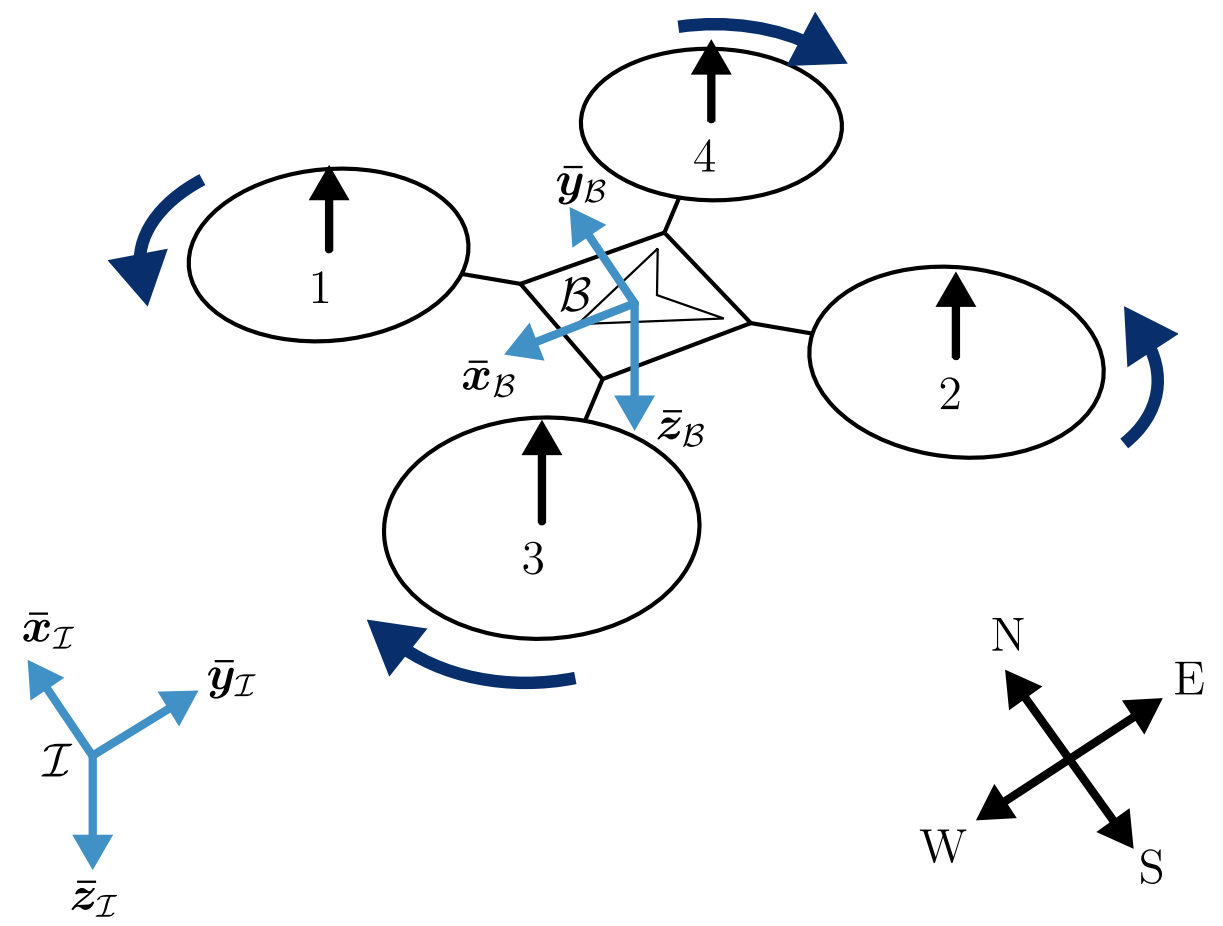
\includegraphics[width=0.6\linewidth]{modelling/fig/coord_frames}
        \caption{Inertial and body coordinate frames of a quadrotor from \cite{Erasmus2020}}
        \label{fig:coord_frames}
    \end{figure}

    \paragraph
    The inertial frame is denote by $ \mathcal{I} = \{ \bm{\bar{x}}_\mathcal{I}, \bm{\bar{y}}_\mathcal{I}, \bm{\bar{z}}_\mathcal{I} \} $ and describes a \gls{NED} axis system.
    The $x$, $y$, and $z$ axis, align with the North, East, and Down inertial directions respectively.
    The inertial frame assumes a flat, non-rotating earth, since the quadrotor will travel small distances in comparison to the curvature of the earth.
    The origin of this frame is fixed at the takeoff location of the multirotor.

    \paragraph
    The body frame is denote by $ \mathcal{B} = \{ \bm{\bar{x}}_\mathcal{B}, \bm{\bar{y}}_\mathcal{B}, \bm{\bar{z}}_\mathcal{B} \} $ and is fixed to the quadrotor body.
    The origin of this frame is at the \gls{CoM} of the vehicle and the $x$, $y$, and $z$ axis, align with the forwards, rightwards, and downwards directions of the quadrotor body respectively.
    The body frame is defined by a translation and rotation relative to the inertial frame.
    The position of the \gls{CoM} of the multirotor in the inertial frame is denoted as $P = [P_N~~P_E~~P_D]^T$. 
    This represents the translation of the body frame relative to the inertial frame.
    The rotations will be discussed in the section below.

\FloatBarrier\section{Rotations}
    
    \paragraph
    The rotation of the body frame relative to the inertial frame can also be referred to as the attitude of the multirotor.
    This can be defined in terms of Euler angles or quaternions.

    \FloatBarrier\subsection{Euler angles}

        \paragraph
        Euler angles are a popular way of describing a \gls{3D} rotation as a sequence of three consecutive elementary rotations \cite{Brescianini2013}.
        For aircraft applications, the ZYX-sequence is common \cite{Brescianini2013} and will be used in this work.
        The order of rotations are:
        \begin{enumerate}
            \item Rotate the body frame about the $z$-axis by the yaw angle, $\Psi$.
            \item Rotate the resulting frame about the new $y$-axis by the pitch angle, $\Theta$.
            \item Rotate the resulting frame about the new $x$-axis by the roll angle, $\Phi$.
        \end{enumerate}

        \begin{figure}[!htbp]
            \centering
            \vspace{0.5cm}
            \def\svgwidth{\columnwidth}
            \scalebox{1.0}{\input{modelling/fig/Euler_rotations.pdf_tex}}
            \caption{Illustration of Euler angles from \cite{Slabber2020}}
            \label{fig:Euler_rotations}
        \end{figure}

        \paragraph
        Figure~\ref{fig:Euler_rotations} gives a simple illustration of the Euler ZYX angles.
        Note that $\Theta$ and $\Phi$ are each illustrated as a pure pitch angle and roll angle from the the inertial frame, without a prior Euler rotation.

    \FloatBarrier\subsection{Quaternions}

        \paragraph
        introduce


\FloatBarrier\section{Multirotor with a suspended payload}

    \paragraph
    The suspended payload is modelled as a rigid body attached by a link to the \gls{CoM} of the quadrotor rigid body.
    Figure~\ref{fig:quad_payload} illustrates a quadrotor with a suspended payload.
    The Euler ZYX angles of the suspended payload in the inertial frame are also shown.
    The $x$-axis and $y$-axis Euler angles are denoted by $\theta_p$ and $\phi_p$ respectively.
    The $z$-axis Euler angle does not contribute to the system dynamics and is omitted. 

    \begin{figure}[!htbp]
        \centering
        \def\svgwidth{\columnwidth}
        \scalebox{0.6}{\input{modelling/fig/quad_payload.pdf_tex}}
        \caption{Schematic of a quadrotor with suspended payload from \cite{Slabber2020}}
        \label{fig:quad_payload}
    \end{figure}
    
    The following assumptions are made regarding the payload model:
    \begin{itemize}
        \item The payload is a point mass.
        \item The link is massless.
        \item The link is rigid.
        \item The link is attached to the \gls{CoM} of the multirotor.
    \end{itemize}

    \paragraph
    The payloads used in the practical setup and described in Chapter~\ref{chap:exp_design}, 
    are small relative to the quadrotor and the attachment point is close to the payload \gls{CoM}.
    They are attached with a low-friction swivel to the suspended cable, therefore the rotation of the payload around the cable axis has a negligible effect on the quadrotor. 
    Therefore modelling a payload as a point mass seems reasonable.

    \paragraph
    The cables used in Chapter~\ref{chap:exp_design} have a very low mass in comparison to the payloads and have a negligible amount of stretch.
    Furthermore, the cable remains straight and rigid during flight due to the tension applied by the payload.
    Aggressive flights may cause periods of zero cable tension where the load is in free-fall and the cable is slack \cite{Tang2015}.
    However, such aggressive manoeuvres will not be considered in this work and the assumption of a rigid, massless cable appears reasonable.

    \paragraph
    In the practical setup shown in Chapter~\ref{chap:exp_design}, the cable is attached appears to be very near to the \gls{CoM} of the quadrotor.
    It is assumed that if the attachment point is slightly below this point it will have a negligible effect on the dynamics.

\FloatBarrier\section{Forces and moments}

    \paragraph
    damping of payload angle


\FloatBarrier\section{Lagrangian mechanics}
    \begin{enumerate}
        \item Discuss weak link between altitude dynamics and swing angle
    \end{enumerate}


\FloatBarrier\section{Model verification} \label{sec:model_verification}

    \paragraph
    Intro

    \begin{figure}[htb]
    \centering
    \begin{tikzpicture}
        \begin{axis}[            
            xlabel = Time,
            ylabel = North velocity,
            x unit = \si{\second},
            y unit = \si{\metre/\second},
            xmin = 0,   xmax = 16,
            ymin = -0.1,  ymax = 2.5,
            grid = major,
            legend cell align = left,
            legend pos = south east,
            grid style = dashed,
            legend style = {font = \scriptsize},
            label style = {font = \scriptsize},
            tick label style = {font = \scriptsize},
            width = 0.95\columnwidth,
            height = 0.5\columnwidth,
            % initialize Dark2
            cycle list/Dark2,
            % combine it with 'mark list*':
            cycle multiindex* list = {
                Dark2\nextlist
            }
        ]
                
        \addplot+[mark = none, style = solid, ultra thick] 
        table[x = time, y = vel_sp, col sep = comma] 
        {modelling/csv/prac_vs_sim_vel_step_Simulink_2021-08-20_04_no_load_velocity_steps_wind_0.5.csv.csv};
        \addlegendentry{$V_{N_{sp}}$}

        \addplot+[mark = none, style = solid, ultra thick] 
        table[x = time, y = vel.prac, col sep = comma] 
        {modelling/csv/prac_vs_sim_vel_step_Simulink_2021-08-20_04_no_load_velocity_steps_wind_0.5.csv.csv};
        \addlegendentry{$V_N$ (Practical)}

        \addplot+[mark = none, style = dashed, ultra thick] 
        table[x = time, y = vel.sim, col sep = comma] 
        {modelling/csv/prac_vs_sim_vel_step_Simulink_2021-08-20_04_no_load_velocity_steps_wind_0.5.csv.csv};
        \addlegendentry{$V_N$ (Simulated)}

        \end{axis}
    \end{tikzpicture} 
    \caption{Comparison of simulated and practical data from Honeybee.}
    \label{fig:prac_vs_sim_vel_step_no_payload}
\end{figure}


    \paragraph
    No load

    \begin{figure}[htb]
    \centering
    \begin{tikzpicture}
        \begin{axis}[            
            xlabel = Time,
            ylabel = North velocity,
            x unit = \si{\second},
            y unit = \si{\metre/\second},
            xmin = 0,   xmax = 16,
            ymin = -0.1,  ymax = 2.8,
            grid = major,
            legend cell align = left,
            legend pos = south east,
            grid style = dashed,
            legend style = {font = \scriptsize},
            label style = {font = \scriptsize},
            tick label style = {font = \scriptsize},
            width = 0.95\columnwidth,
            height = 0.5\columnwidth,
            % initialize Dark2
            cycle list/Dark2,
            % combine it with 'mark list*':
            cycle multiindex* list = {
                Dark2\nextlist
            }
        ]
                
        \addplot+[mark = none, style = solid, ultra thick] 
        table[x = time, y = vel_sp, col sep = comma] 
        {modelling/csv/prac_vs_sim_vel_step_Simulink_2021-08-20_02_l-2_mp-0.3-wind-0.5.csv.csv};
        \addlegendentry{$V_{N_{sp}}$}

        \addplot+[mark = none, style = solid, ultra thick] 
        table[x = time, y = vel.prac, col sep = comma] 
        {modelling/csv/prac_vs_sim_vel_step_Simulink_2021-08-20_02_l-2_mp-0.3-wind-0.5.csv.csv};
        \addlegendentry{$V_N$ (Practical)}

        \addplot+[mark = none, style = dashed, ultra thick] 
        table[x = time, y = vel.sim, col sep = comma] 
        {modelling/csv/prac_vs_sim_vel_step_Simulink_2021-08-20_02_l-2_mp-0.3-wind-0.5.csv.csv};
        \addlegendentry{$V_N$ (Simulated)}

        \end{axis}
    \end{tikzpicture} 
    \caption{Velocity step comparison of simulated and practical data for Honeybee with a suspended payload.}
    \label{fig:prac_vs_sim_vel_step_with_payload}
\end{figure}


    \paragraph
    With payload vel

    \begin{figure}[htb]
    \centering
    \begin{tikzpicture}
        \begin{axis}[            
            xlabel = Time,
            ylabel = Payload angle,
            x unit = \si{\second},
            y unit = \si{\degree},
            xmin = 0,   xmax = 16,
            ymin = -20,  ymax = 20,
            grid = major,
            legend cell align = left,
            legend pos = south east,
            grid style = dashed,
            legend style = {font = \scriptsize},
            label style = {font = \scriptsize},
            tick label style = {font = \scriptsize},
            width = 0.95\columnwidth,
            height = 0.5\columnwidth,
            % initialize Dark2
            cycle list/Dark2,
            % combine it with 'mark list*':
            cycle multiindex* list = {
                Dark2\nextlist
            }
        ]
                
        \addplot+[mark = none, style = solid, ultra thick] 
        table[x = time, y = theta.prac, col sep = comma] 
        {modelling/csv/prac_vs_sim_vel_step_Simulink_2021-08-20_02_l-2_mp-0.3-wind-0.5.csv.csv};
        \addlegendentry{Practical}

        \addplot+[mark = none, style = dashed, ultra thick] 
        table[x = time, y = theta.sim, col sep = comma] 
        {modelling/csv/prac_vs_sim_vel_step_Simulink_2021-08-20_02_l-2_mp-0.3-wind-0.5.csv.csv};
        \addlegendentry{Simulated}

        \end{axis}
    \end{tikzpicture} 
    \caption{Payload angle comparison of simulated and practical data for Honeybee with a suspended payload}
    \label{fig:prac_vs_sim_theta_with_payload}
\end{figure}


    \paragraph
    With payload theta



    \begin{enumerate}
        \item Plot velocity step
        \item Plot position step
    \end{enumerate}

\FloatBarrier\section{Linearised model}
    \label{sec:linear_model}

\FloatBarrier\section{Dynamic payloads}

    In this work, a dynamic payload refers to a payload with dynamics that differ significantly from a rigid mass.
    When considering suspended payloads, a dynamic payload induces dynamics which differ from that of a simple pendulum.

    \begin{itemize}
        \item Most control in literature model payload as rigid Mass. Give references.
        \item Some add spring stiffness of cable (give references e.g. QuadLoad ElasticCable Prasanth Kotaru)
        \item but not practical because can design which cable you used. Cannot design which payload needs to be transported
        \item water looks like double payload
    \end{itemize}
% https://hybrid-robotics.berkeley.edu/publications/ACC2017_QuadLoad_ElasticCable.pdf), 
% https://www.researchgate.net/publication/352394086_A_Hybrid_Control_Approach_for_the_Sw[…]=publicationTitle&_iepl%5BtargetEntityId%5D=PB%3A352394086

}


% \graphicspath{{system_id/fig/}}

\chapter{System identification}
\label{chap:system_id}

    \paragraph{}
    System identification is the process of creating mathematical models of a dynamical system by using input and output measurements of that system.
    Two major approaches are used to represent the dynamics of such a system:
    \begin{enumerate}
        \item A priori mathematical modelling with parameter estimation
        \item Data-driven system identification
    \end{enumerate}

    Models determined from a priori modelling and parameter estimation are referred to as white-box models.
    In contrast, data-driven system identification methods result in black-box models.
    This chapter discusses these system identification approaches and describes the differences between them.
    For each approach, different estimation techniques are explained and applied to the quadrotor and payload system.
    The results of these techniques are then compared to each other.    

\section{White-box and black-box techniques}

    \subsection{White-box techniques}

        \paragraph{} 
        The underlying physics of a white-box model is understood by the user because    
        they are determined from first principles.
        This is done by modelling physical processes with techniques like Lagrangian mechanics or Newton equations.
        With system identification techniques that use these models, 
        the mathematical relations between system parameters are predefined in the modelling phase.
        The system identification process is therefore reduced to parameter estimation to determine values for parameters used in die model.

        \paragraph{} 
        This approach is used by \cite{Erasmus2020} and \cite{Slabber2020} for swing damping control of a quadrotor with an unknown suspended payload.
        The system was modelled as two rigid bodies connected by a link and the following assumptions were made regarding the suspended payload:
        \begin{itemize}
            \item The payload is a point mass.
            \item The link is massless.
            \item The link is rigid.
            \item The link is attached to the CoM of the quadrotor.
        \end{itemize}
        The only unknown parameters in the quadrotor and payload model is the payload mass and link length.
        These parameters are first estimated and then inserted into the predefined, linearised model.
        This model is used by a LQR controller to damp swing angles while also controlling the vehicle.

        \paragraph{} 
        The approach works well for systems with predictable dynamics, but it is not very adaptable.
        The payload considered by \cite{Erasmus2020} and \cite{Slabber2020} is limited to a small rigid mass suspended from the quadrotor by a non-stretching cable. 
        In this use case it was shown that a LQR controller successfully controls a quadrotor while minimising payload swing angles.
        However, if a payload or cable is used that violates one of the modelling assumptions, the predefined model no longer accurately represent the system.
        Since the controller is dependent on this model, the mismatch between the model and actual dynamics may result in undesirable controller behaviour.

    \subsection{Black-box techniques}

        Data-driven system identification methods produce black-box models.
        In contrast to white-box models, black-box models do not require predefined mathematical relations between system parameters.
        % The user only considers what goes into, and comes out of, the black-box.
        % Something imagery about why it is called black box
        No prior knowledge of the physics of the system are considered and no modelling assumptions are made.
        Black-box techniques determine the mathematical relationship between inputs and outputs of a system using information from measurement data only.

        \paragraph{}
        Black-box models can be categorised as either non-linear or linear models.
        Non-linear models are often more accurate than linear models because complex, real-world dynamics are better approximated by non-linear systems.
        The dynamics of a quadrotor and suspended payload are also non-linear.
        Examples of black box models with quadrotors and payloads in literature ???

        \paragraph{}
        However, non-linear models are inherently more complex than linear models. 
        Controllers that use non-linear models are usually more computationally complex than those with linear models.
        Control archetictures for quadrotors used in practical applications are mostly implemented on onboard hardware.
        Therefore there is value in low-complexity, linear models since these may be simple enough to execute on low cost hardware.
        trade-off between accuracy and complexity.
        Non-linear models may require control implementations that are too computationally expensive and may not be practically realisable on the available hardware on a quadrotor.
        
        \paragraph{}
        DMDc and HAVOK are the two data-driven system identification methods investigated in this paper. 
        These are linear regression techniques that produce a linear model to approximate non-linear dynamics.
        Non-linear data-driven techniques like Neural Networks and SINDy \cite{Brunton2016} may produce models that are more accurate than linear techniques, 
        but at the cost of greater computational complexity.
        \murray{Name more techniques}
        DMDc and HAVOK are less computationally complex and their models are suitable for linear MPC, which is significantly faster than non-linear MPC.
        This is desirable for the quadrotor use case, where onboard computational power is limited.
        
        \paragraph{}
        These techniques and their implementation are explained in the sections below.
        Each technique is considered for use in a velocity controller in the North direction

        \paragraph{Considered controller}
        % As discussed in \ref{sec:linear_model}, the payload has minimal effect on quadrotor attitude because it is attached near the CoM of the vehicle.
        % Therefore the attitude states are excluded from the system identification model.
        The model identified by DMDc will be used to design a longitudinal velocity controller.
        As shown in \ref{fig:system_id_plant}, the plant considered for system identification includes the dynamics of the inner loop, attitude controllers.
        The swing damping controllers which will utilise the identified model act only in the translational velocity loop.
        Because of the large time-scale separation between the inner and outer loop controllers, 
        the attitude states have a negilable effect on the plant dynamics seen by the velocity controller.
        As discussed in Section~\ref{sec:linear_model}, the payload minimally effects the quadrotor attitude because it is attached near the CoM of the vehicle.
        Therefore the attitude states are excluded from the system identification model.

\section{Plant considered for system identification}
        \begin{figure}[h]
            \centering
        %     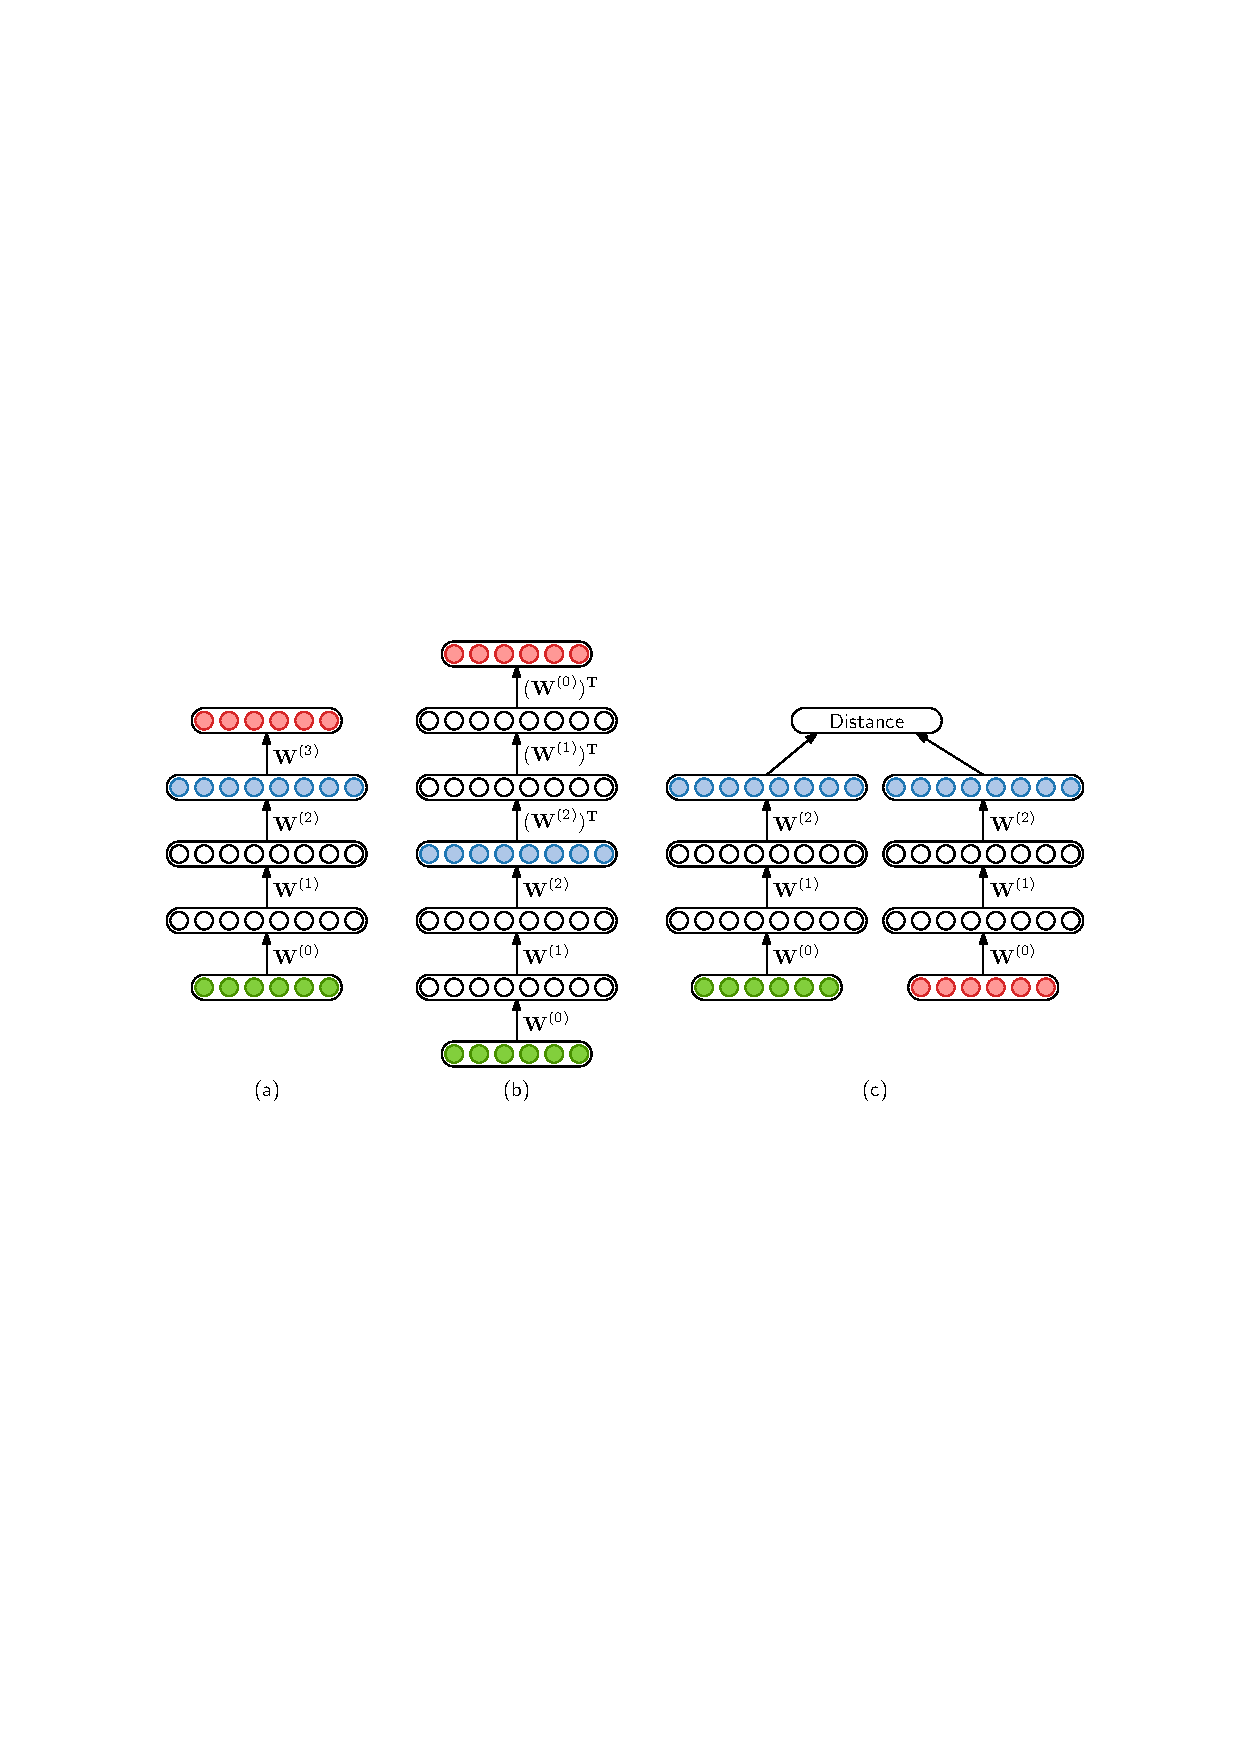
\includegraphics[width=\linewidth]{cae_siamese}
            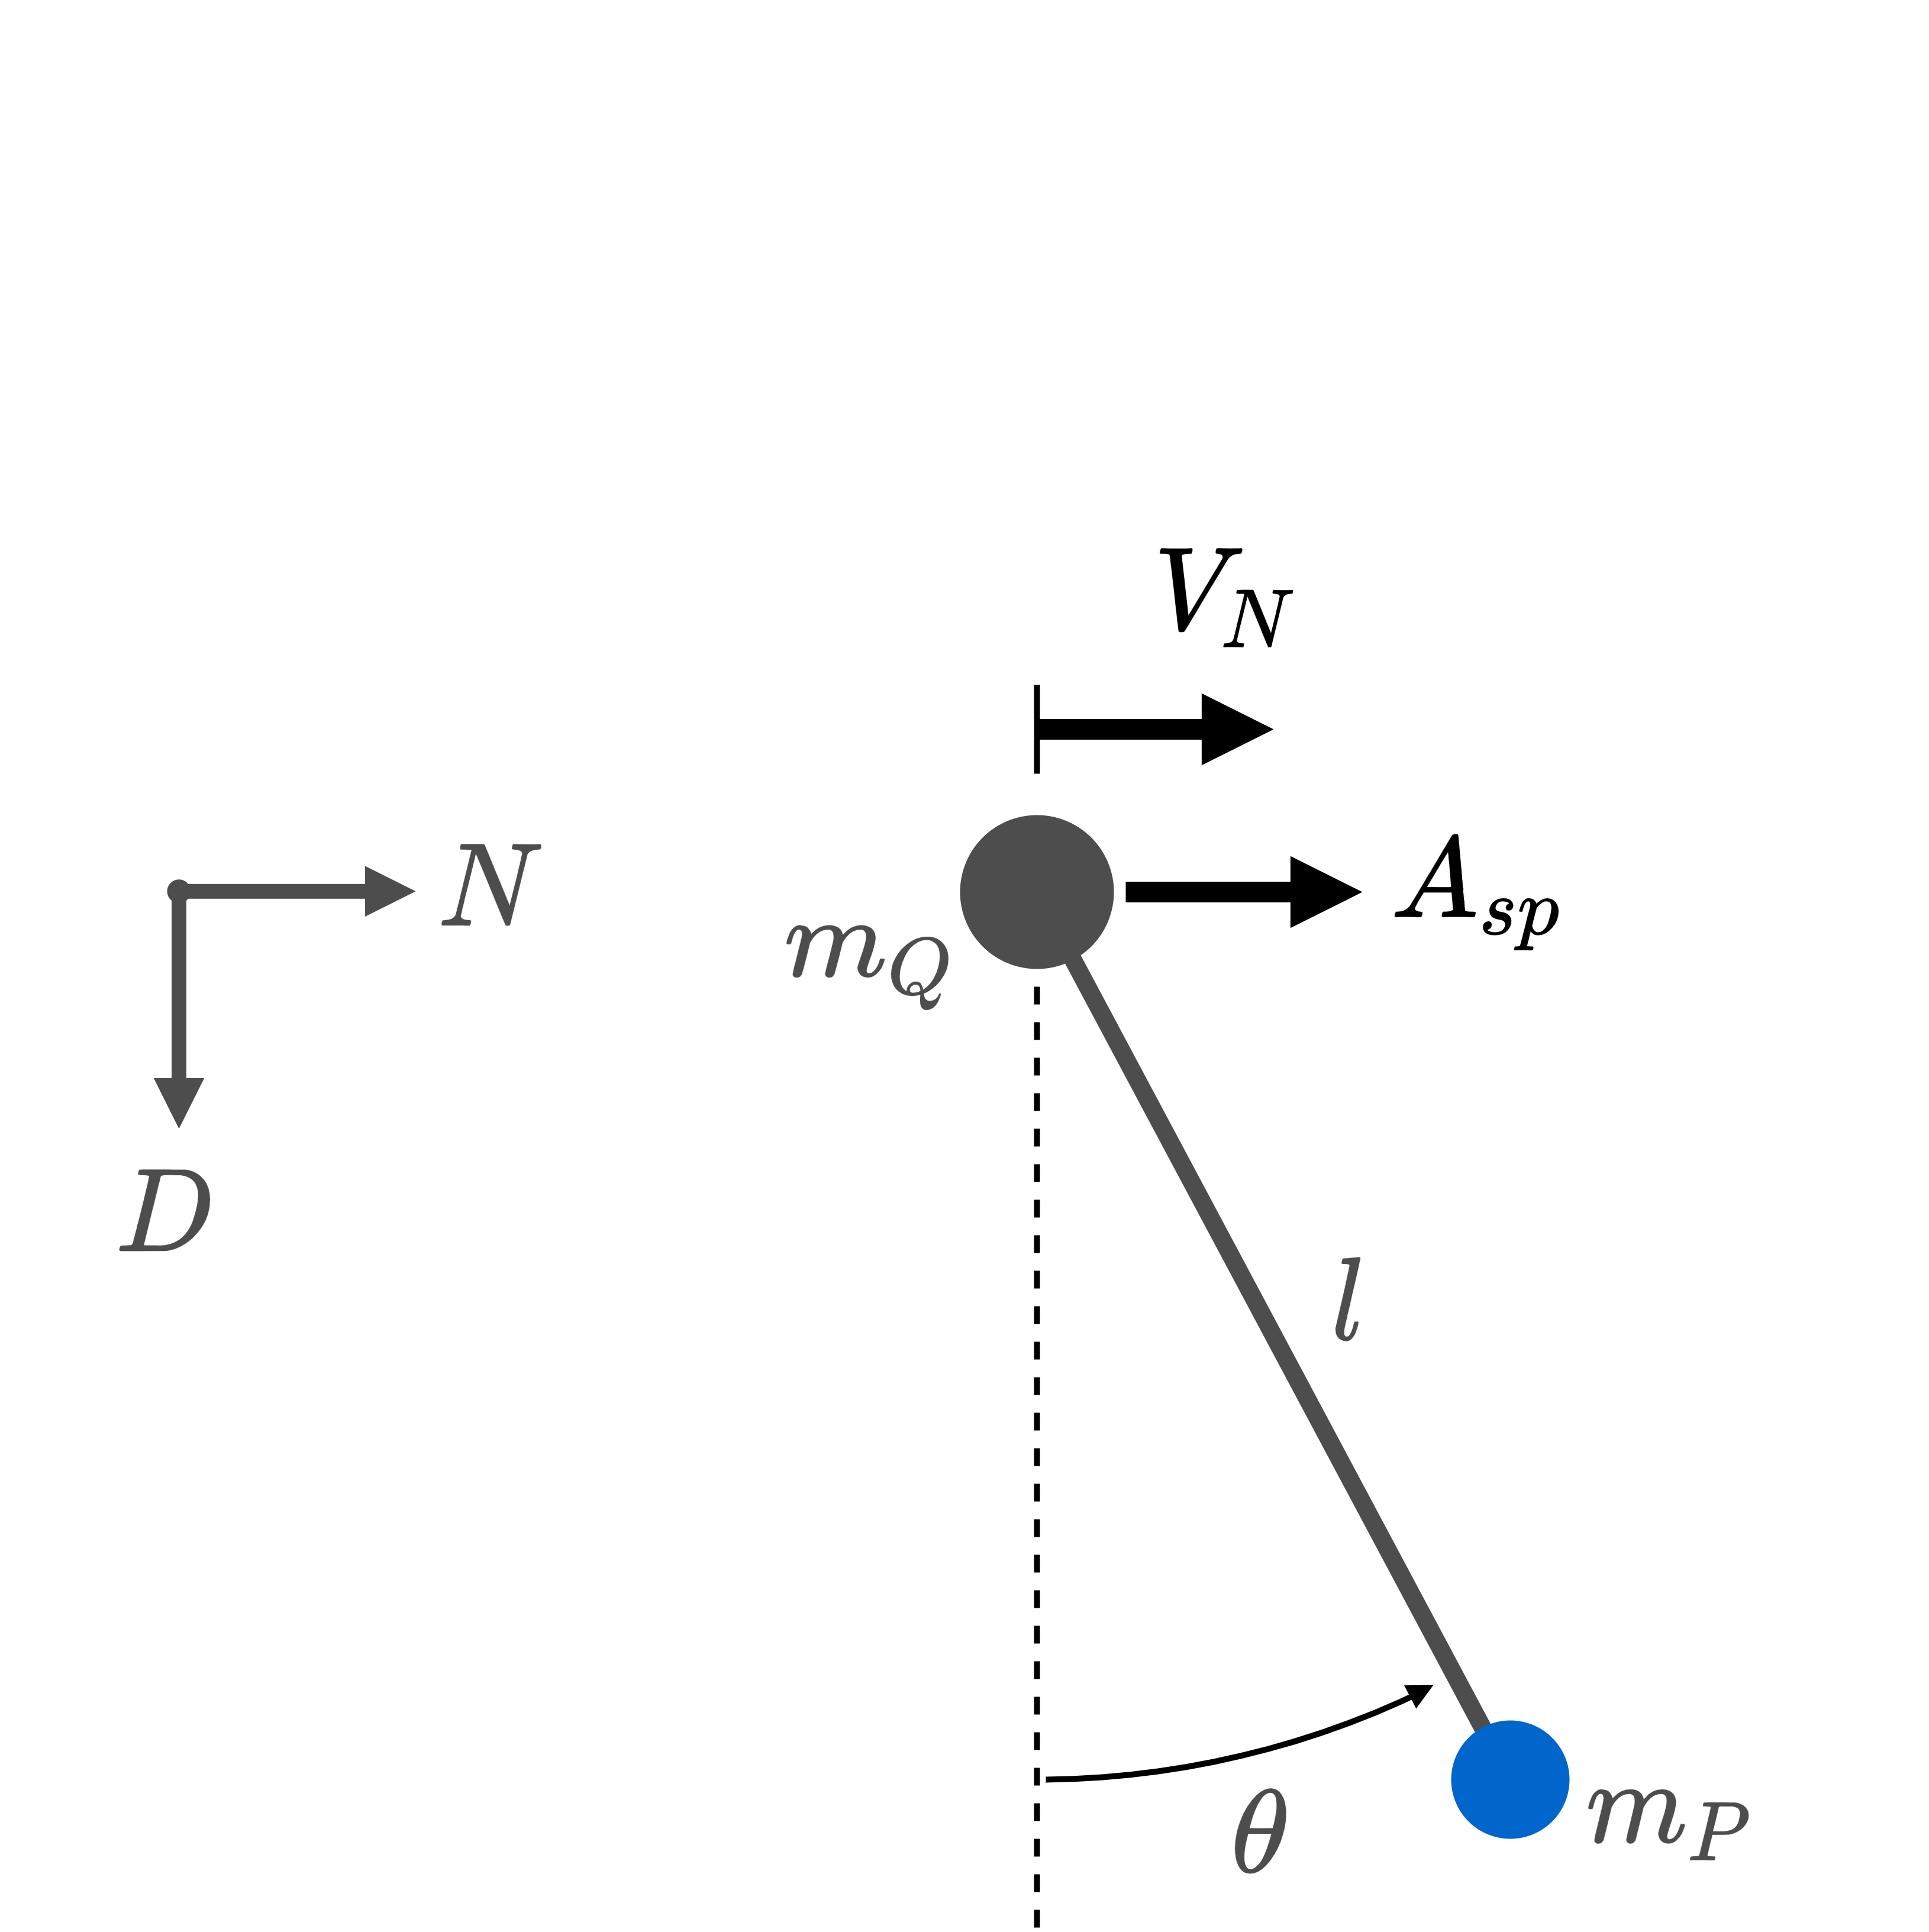
\includegraphics[width=0.5\linewidth]{floating_pend.png}            
            \caption{Floating pendulum model considered for system identification for a North velocity controller}
            \label{fig:floating_pend}
        \end{figure}
    
        \paragraph{Derived model}
        Figure \ref{fig:floating_pend} shows the plant considered for system identification.
        In Chapter~\ref{chap:modelling} the differential equations that describe the motion of this system are derived with Lagrangian mechanics.
        From these equations it is clear that the considered plant is defined by the state vector,
        \begin{equation}
            \bm{x} = \begin{bmatrix}
                V_N & \dot{\theta}
            \end{bmatrix}^T,
        \end{equation}
        and the input vector,
        \begin{equation}
            \bm{u} = \begin{bmatrix}
                A_{N,sp}
            \end{bmatrix},
        \end{equation}
    
        % From this derivation it is clear that the angular velocity of the payload, $\dot{\theta}$, is required to described the system dynamics.
        % However, $\dot{\theta}$ is not measured directly on the considered practical quadrotor setup.
        % Instead, the payload angle, $\theta$, is measured by a potentiometer attached to a ADC on Honeybee as described in Chapter \ref{chap:system_overview}.
        % As expected, this measurement is extremely noisy.
        % \murray{Maybe insert figure to show noise}
        % % Figure \ref{} shows the angle measurement during a practical experiment of the payload while Honeybee is held stationary
        % Numerical differentiation is applied to the noisy $\theta$ signal which results in a very inaccurate estimation of $\dot{\theta}$.
        % Therefore it is desirable to rather use $\theta$ in the system identification process. 

\section{Parameter estimation}
    \subsection{Predetermined linear model}
        The motivation for paramater estimation is to determine unknown parameter values required by the predetermined model.
        This model was derived a prioiri in Section~\ref{sec:linear_model}.
        
    \subsection{Payload mass estimation}
        RLS

    \subsection{Cable length estimation}
        The cable length is estimated from the measurement of natural frequency of the swinging payload.
        As described by
        \cite{bisgaard},
        the natural frequency is given by:
        \begin{equation} \label{eq:nat_freq}
            \omega_n = \sqrt{ \frac{g}{l} \cdot \frac{m_q + m_p}{m_q}}
        \end{equation}
        The natural frequency is measured by performing a FFT on the payload swing angle response after a position step by the quadrotor.
        The dominant frequency identified by the FFT during free swing is the natural frequency of the payload.
        
        \ref{fig:pos_step_angle}
        shows the payload swing angle after the system is stimulated by a position step setpoint.
        As shown in 
        \ref{fig:pos_step_angle}
        the first few seconds of the step response are not used in the FFT.
        This is to minimise the effect of the quadrotor controllers on the swing angle frequency 
        by excluding the transient response in the FFT.

        \ref{fig:fft} 
        shows the resulting amplitude spectrum of the payload swing angle response.
        The dominant frequency is clearly identified as ??.
        Since $m_q$ and $g$ is known, and $m_p$ and $\omega_n$ has been estimated, $l$ can now be determined from
        \ref{eq:nat_freq}.
        In this case the estimated length is ??, compared to the actual length of ??.
        
        Frequency resolution ??
        error for different lengths??
  
\section{Dynamic Mode Decomposition with control}
\label{sec:dmdc}
    
    \paragraph{Intro}        
    DMD is a linear regression technique that can be used to approximate a non-linear dynamical system \cite{Tu2014}.
    It uses temporal measurements of system outputs to reconstruct system dynamics without prior modelling assumptions.
    DMDc is an adaptation of DMD that also accounts for control inputs \cite{Proctor2016c}.
    This section provides an overview of the specific implementation of DMDc used in this paper.        
    Note that this implementation is a slight adaptation of DMDc, and includes time-delay-embedding of multiple observables. 
    \cite{Korda2018b} and \cite{Arbabi2018} use time-delay-embedding in their DMD adaptions in similar ways.

    \paragraph{State space model}
    DMD produces a linear, discrete state-space model of the system dynamics.
    Discrete measurements, $\bm{x}_k$, of the continuous time observable, $\bm{x}(t)$, are used, 
    where $\bm{x}_k = \bm{x}(k T_s)$, and $T_s$ is the sampling time of the model.    
    Delay-coordinates (i.e. $\bm{x}_{k-1}, \bm{x}_{k-2}$, etc.) are also included in the state-space model to
    account for input delay and state delay in the system.
    Input delay refers to the time delay involved with transporting a control signal to a system, 
    whereas state delay refers to time-separated interactions between system variables \cite{Chen1999}.
    Hence, we define an state delay vector as:
    \begin{equation}
        \bm{d}_{k} = 
        \begin{bmatrix}
            \bm{x}_{k-1} & \bm{x}_{k-2} & \cdots & \bm{x}_{k-q}
        \end{bmatrix}^T ,
    \end{equation}
    $\bm{d}_k \in \R^{(n_x)(q)}$ and where $q$ is the number of delay-coordinates used in the model.
    
    \paragraph{}
    The discrete state-space model is therefore defined as:
    \begin{equation} \label{eq:dmd_state_space}
        \bm{x}_{k+1} = \bm{A} \bm{x}_k + \bm{A}_d \bm{d}_k + \bm{B} \bm{u}_k ,
    \end{equation}
    \( \bm{A} \in \R^{n_x \times n_x} \) is the system matrix, 
    \( \bm{A}_1 \in \R^{(q \cdot n_x) \times (q \cdot n_x)} \) is the state delay system matrix and 
    \( \bm{B} \in \R^{n_x \times n_u} \) is the input matrix.
    
    \paragraph{Training data}
    The training data consists of full-state measurements, $\bm{x}_k$, and corresponding inputs, $\bm{u}_k$, 
    taken at regular intervals of $\Delta t = T_s$, during a simulated flight with Cascaded PID control.
    In a practical flight, these time-series measurements need to be saved in memory because it is usd as a single batch by DMD.
    Note that DMD can be applied in a recursive manner as described in \cite{Noack2016}, 
    However this implementation is not considered because memory size will not be a limitation since a companion computer will be used.
    
    \paragraph{Data matrices}
    The training data is collected into the following matrices:
    \begin{align} \label{eq:dmd_matrices}
        \bm{X^\prime} = & \phantom{.} \left [
            \begin{array}{*{5}{@{}M{\mycolwd}@{}}}
                    \bm{x}_{q+2} & \bm{x}_{q+3} & \bm{x}_{q+4} & \cdots & \bm{x}_{w+q+1}
            \end{array}
        \right ] , \nonumber \\
        %
        \bm{X} \phantom{''} = & \phantom{.} \left [
            \begin{array}{*{5}{@{}M{\mycolwd}@{}}}
                \bm{x}_{q+1} & \bm{x}_{q+2} & \bm{x}_{q+3} & \cdots & \bm{x}_{w+q}                      
            \end{array}
        \right ] , \nonumber \\
        % 
        \bm{X}_d \phantom{'} = & \phantom{'} \left [
            \begin{array}{*{5}{@{}M{\mycolwd}@{}}}
                \bm{x}_{q} & \bm{x}_{q+1} & \bm{x}_{q+2} & \cdots & \bm{x}_{w+q-1} \\
                \vdots   & \vdots   & \vdots   & \ddots & \vdots \\
                \bm{x}_2 & \bm{x}_3 & \bm{x}_4 & \cdots & \bm{x}_{w+1} \\
                \bm{x}_1 & \bm{x}_2 & \bm{x}_3 & \cdots & \bm{x}_{w} \\                       
            \end{array}
        \right ] , \nonumber \\
        % 
        \bm{\Upsilon} \phantom{'} = & \phantom{.} \left [
            \begin{array}{*{5}{@{}M{\mycolwd}@{}}}
                    \bm{u}_{q} & \bm{u}_{q+1} & \bm{u}_{q+2} & \cdots & \bm{u}_{w+q-1}
            \end{array}
        \right ] ,
    \end{align}

    where $w$ is the number of columns in the matrices, 
    $\bm{X^\prime}$ is the matrix $\bm{X}$ shifted forward by one time-step, 
    $\bm{X}_d$ is the matrix with delay states, 
    and $\bm{\Upsilon}$ is the matrix of inputs.
    Equation (\ref{eq:dmd_state_space}) can be combined with the matrices in Equation (\ref{eq:dmd_matrices}) to produce:
    \begin{equation}
        \bm{X^\prime} = \bm{A} \bm{X} + \bm{A}_d \bm{X}_d + \bm{B} \bm{\Upsilon} .
    \end{equation}
    Note that the primary objective of DMDc is to determine the best fit model matrices, $\bm{A}$, $\bm{A}_d$ and $\bm{B}$, 
    given the data in $\bm{X^\prime}$, $\bm{X}$, $\bm{X}_d$, and $\bm{\Upsilon}$ \cite{Proctor2016c}.
    In order to group the unknowns into a single matrix, (\ref{eq:dmd_state_space}) is manipulated into the form,
    \begin{equation} \label{eq:G_Omega}
        \bm{X^\prime} =   
        \begin{bmatrix} 
            \bm{A} & \bm{A}_d & \bm{B} 
        \end{bmatrix}
        \begin{bmatrix} 
            \bm{X} \\ \bm{X}_d \\ \bm{\Upsilon} 
        \end{bmatrix} 
        = \bm{G \Omega} ,
    \end{equation} 
    where $\bm{\Omega}$ contains the state and control data, and $\bm{G}$ represents the system and input matrices.
    
    \paragraph{SVD}
    A SVD is performed on $\bm{\Omega}$ resulting in:
    \(
        \bm{\Omega} = \bm{U} \bm{\Sigma} \bm{V}^T
    \).
    Often, only the first $p$ columns of $\bm{U}$ and $\bm{V}$ are required for a good approximation of the dynamics \cite{Brunton2017a}.
    In many cases, the truncated form results in better models than the exact form when noisy measurements are used.
    This is because the effect of measurement noise is mostly captured by the truncated columns of $\bm{U}$ and $\bm{V}$.
    By truncating these columns, the influence of noise in the regression problem is reduced. \murray{explain this better}
    hence the SVD is used in the truncated form: 
    \begin{equation} \label{eq:tilde_svd}
        \bm{\Omega} \approx \Tilde{\bm{U}} \Tilde{\bm{\Sigma}} \Tilde{\bm{V}}^T ,
    \end{equation}
    where $\phantom{.} \Tilde{ } \phantom{.}$ represents rank-$p$ truncation.
    \murray{maybe insert colour pictures showing matrices}        

    \paragraph{}
    By combining (\ref{eq:tilde_svd}) with the over-constrained equality in (\ref{eq:G_Omega}), 
    the least-squared solution, $\bm{G}$, can be found with:
    \begin{equation}
        \bm{G} \approx \bm{X^\prime} \Tilde{\bm{V}} \Tilde{\bm{\Sigma}}^{-1} \Tilde{\bm{U}} .
    \end{equation}
    By reversing \ref{eq:G_Omega}, $\bm{G}$ can now be separated into:
    \(
        \bm{G} = \begin{bmatrix} \bm{A} & \bm{A}_d & \bm{B} \end{bmatrix}.
    \)
    according to the required dimensions of each matrix.
    Thereby, the state-space model approximated by DMDc is complete.
    
\section{Hankel Alternative View Of Koopman}
    
    \murray{q = number of delays, from here up}
    
    \paragraph{}
    HAVOK is a data-driven, regression technique that provides a connection between DMD and Koopman operator theory \cite{Brunton2017a, Champion2019}. 
    We have adapted the standard HAVOK algorithm slightly to account for the effect of control and to extract a discrete, linear model that approximates the behaviour of a controlled dynamical system.
    In this section, a brief overview is provided for this implementation and expansion of \mbox{HAVOK}.
    % 
    \paragraph{}
    The extracted discrete state-space model is defined as:
    \begin{equation} \label{eq:havoc_state_space}
        \bm{a}_{k+1} = \Tilde{\bm{A}} \bm{a}_k + \Tilde{\bm{B}} \bm{u}_k ,
    \end{equation}
    where $\bm{a}_k$ is the state vector previously defined in Section \ref{sec:dmdc}, 
    \( \Tilde{\bm{A}} \in \R^{(q \cdot n_x) \times (q \cdot n_x)} \) is the system matrix, 
    and \( \Tilde{\bm{B}} \in \R^{(q \cdot n_x) \times n_u} \) is the input matrix. 
    Here, $\Tilde{\phantom{a}}$ is used to differentiate these matrices from $\bm{A}$ and $\bm{B}$ used in DMDc.
    % 
    \paragraph{}
    The original HAVOK algorithm, developed by \cite{Brunton2017}, constructs a Hankel matrix from output variables only. 
    In order to incorporate the effect of control, an extended Hankel matrix, $\bm{\Pi}$, is created by appending a matrix of inputs to a Hankel matrix of measurements:
    \begin{equation} \label{eq:pi_hankel}
        \bm{\Pi} = \phantom{.} \left [
            \begin{array}{*{5}{@{}M{\mycolwd}@{}}}
                    \bm{a}_{q} & \bm{a}_{q+1} & \bm{a}_{q+2} & \cdots & \bm{a}_{w+q-1} \\
                    \bm{u}_{q} & \bm{u}_{q+1} & \bm{u}_{q+2} & \cdots & \bm{u}_{w+q-1}
            \end{array}
        \right ] ,
    \end{equation}
    where $w$ is the number of columns in $\bm{\Pi}$.
    A truncated SVD of this Hankel matrix results in following approximation:
    \begin{equation} \label{eq:havok_svd_tilde}
        \bm{\Pi} \approx \Tilde{\bm{U}} \Tilde{\bm{\Sigma}} \Tilde{\bm{V}}^T ,
    \end{equation}
    where $\Tilde{\phantom{a}}$ represents rank-$p$ truncation.
    It is important to note that the model extracted by HAVOK depends on the choice of hyperparameters, $p$ and $q$.
    The number of samples in the training data, $N_{train} = w + q -1$, also influences the accuracy of the model.
    % 
    \paragraph{}
    The columns of $\Tilde{\bm{V}}$ are the most significant principal components of the system dynamics \cite{Kamb2020}.
    This matrix, $\Tilde{\bm{V}}$, can be considered to contain a time-series of the pseudo-state, $\bm{v}$, such that
    \(
        \Tilde{\bm{V}}^T = \begin{bmatrix} 
            \bm{v}_q & \bm{v}_{q+1} & \cdots & \bm{v}_w 
        \end{bmatrix} ,
    \)
    characterises the evolution of the actual dynamics in an eigen-time-delay coordinate system \cite{Brunton2017}.
    % 
    Consider the following discrete, state-space formulation:
    \begin{equation} \label{eq:v_ss}
        \bm{v}_{k+1} = \bm{\Lambda} \bm{v}_k .
    \end{equation}
    Recall that DMDc finds a best fit linear operator that directly maps $\bm{a}_{k}$ to $\bm{a}_{k+1}$.
    Similarly, HAVOK determines the best fit linear operator $\bm{\Lambda}$ that maps the pseudo-state $\bm{v}_k$ to $\bm{v}_{k+1}$.
    So, in order to setup an over-determined equality for (\ref{eq:v_ss}), $\Tilde{\bm{V}}^T$ is divided into two matrices:
    \begin{align} \label{eq:v1v2}
        \bm{V}_1 &= \left [
            \begin{array}{*{5}{@{}M{\mycolwd}@{}}} 
                \bm{v}_{q \phantom{-1}}     & \bm{v}_{q+1} & ... & \bm{v}_{w-1} \\
            \end{array} 
        \right ] , \nonumber \\ 
        \bm{V}_2 &= \left [
            \begin{array}{*{5}{@{}M{\mycolwd}@{}}} 
                \bm{v}_{q+1}     & \bm{v}_{q+2} & ... & \bm{v}_{w \phantom{-1}} \\
            \end{array} 
        \right ] ,
    \end{align} 
    where $\bm{V}_2$ is $\bm{V}_1$ advanced a single step forward in time.
    The matrices from Equation (\ref{eq:v1v2}) are now combined with Equation (\ref{eq:v_ss}) and the best fit $\bm{\Lambda}$ is determined with the Moore-Penrose pseudoinverse:
    \begin{equation} \label{eq:v_dmd}
        \bm{V}_2 = \bm{\Lambda} \bm{V}_1 \phantom{---} \Rightarrow \phantom{---} \bm{\Lambda} \approx \bm{V}_1 \bm{V}_1^{\dagger}
    \end{equation}
    % 
    It can be shown from Equation (\ref{eq:havok_svd_tilde}) that Equation (\ref{eq:v_ss}) is transformed from the eigen-time-delay coordinate system to the original coordinate system as the following:
    \begin{equation} \label{eq:v_ss_a} 
        \begin{bmatrix}
            \bm{a}_{k+1}  \\  \bm{u}_{k+1} 
        \end{bmatrix}
    \phantom{.} = \phantom{.} (\Tilde{\bm{U}} \Tilde{\bm{\Sigma}}) \bm{\Lambda} (\Tilde{\bm{U}}  \Tilde{\bm{\Sigma}})^{\dagger} \phantom{.}
        \begin{bmatrix}
            \bm{a}_{k}  \\  \bm{u}_{k} 
        \end{bmatrix} .
    \end{equation}    
    % 
    This form is used to extract $\Tilde{\bm{A}}$ and $\Tilde{\bm{B}}$ from the matrix,
    \( 
        (\Tilde{\bm{U}} \Tilde{\bm{\Sigma}}) \bm{\Lambda} (\Tilde{\bm{U}}  \Tilde{\bm{\Sigma}})^{\dagger}
    \), in the following way:
    \begin{equation} \label{matrix_decomp}
        \begin{bmatrix}
            \bm{a}_{k+1}  \\  \bm{u}_{k+1} 
        \end{bmatrix}
        \phantom{.} = \phantom{.} 
        \begin{bmatrix}
            \Tilde{\bm{A}} \phantom{.....} \Tilde{\bm{B}} \\
            \textit{(discarded)}
        \end{bmatrix}
        \phantom{.}
        \begin{bmatrix}
            \bm{a}_{k}  \\  \bm{u}_{k} 
        \end{bmatrix}.
    \end{equation}    
    % 
    % This decomposition is illustrated in Fig.~\ref{fig:lambda_decomp}, where blocks represent different groups of entries in the matrix.
    % \begin{figure}[h]
    %     \includegraphics[scale = 0.45]{Lambda_decomp.png}
    %     \centering
    %     \caption{Illustration of the extraction of $\Tilde{\bm{A}}$ and $\Tilde{\bm{B}}$ from (\ref{eq:v_ss_a})}
    %     \label{fig:lambda_decomp}
    % \end{figure}
    % 
    Note that the matrix entries in (\ref{matrix_decomp}) that map $\bm{u}_k$ to $\bm{u}_{k+1}$ are meaningless for our purposes and are discarded.
    Similarly to DMDc, some matrix entries in $\Tilde{\bm{A}}$ and $\Tilde{\bm{B}}$ are known a priori due to the relative positions of delay coordinates. These are forced to 1 or 0 to improve the prediction performance of the model.
    
    \murray{merge these paragraphs}
    Since the state vector, $\bm{a}$, includes delay-coordinates, some matrix entries are known a priori and are independent of the dynamics. 
    For example, the values of $\bm{x}_{k}$ should be mapped from their position in $\bm{a}_k$ to specific indices in $\bm{a}_{k+1}$. 
    Due to the least-squares fitting and coordinate transformation, DMDc will not produce these exact values in $\bm{A}$ and $\bm{B}$. 
    By forcing each of these matrix entries to 1 or 0, the state-prediction performance of the model is improved.




\section{Implementation and results}
    \subsection{Methodology}
        \paragraph{Simulation environment}

        \paragraph{Method overview}
        \murray{Maybe convert this to a flow diagram}

        \begin{enumerate}
            \item Takeoff and hover
            \item Command a series of velocity step inputs with random step sizes and time intervals
            \item Measure and save input and output data
            \item Apply algorithm to data and generate model
        \end{enumerate}

        \paragraph{}

        \paragraph{Steps and intervals}
        For the training period, different velocity step inputs are commanded with varying time intervals between step commands.
        A algorithm schedules these velocity step commands, by assigning random step values and time-intervals within a specified range.
        The velocity range is determined in simulation by iteratively increasing the maximum velocity step 
        to a safe value where the quadrotor and payload system remain in stable flight.
        The maximum time-interval is set to a value that allows the payload swing to reach a steady-state condition.
        This ensures that the identified model includes transient and steady-state dynamics.

        \paragraph{Why velocity steps?}
        Velocity step commands are used in the training period because this 
        Frequency decomposition stimulates the system for a large range of frequencies.

        \paragraph{Testing data}

        \paragraph{Error metric}
        Each state error signal is scaled by the reciprocal of the maximum value of that state variable in the training data.
        % This is to provide a better representative error when taking the mean of state variable errors.
        This is to ensure that a scale difference in the variable types create a bias in the error metric.
        For example, the quadrotor velocity reaches values of \SI{3}{\metre/\second} but the payload swing angle has a maximum of only \SI[]{0.526}{\radian}.
        The velocity prediction error is therefore inherently larger than the payload angle prediction error
        and will bias the error metric towards favouring models with good velocity predictions.
        The proposed scaled error metric ensures that the MAE of each state variable can be compared to each other.
        It also provides an error metric that is better and unbiased representative of the model prediction performance across all state variables. 

    \subsection{Hyperparameters}
        Fixed size of data
        Fixed sample time
        Fixed pendulum params
        Talk about the "front"
        Also about singular values
        For each of the experiments shown in this chapter, a hyperparameters selected tuned to produced

    \subsection{Sample time}
        best hyperparameters.
        
        Fixed size of data.
        Fixed pendulum params.

    \subsection{Size of training data}
        The length of training data used for system identification also affects the quality of the model produced.
        Figure~\ref{fig:MAE_vs_train} plots the prediciton error metric compared to the length of training data used for the different system identification procedures.
        For each length of training data, the hyperparameter combination producing the lowest prediction error was determined and used.
        From Figure~\ref{fig:MAE_vs_train} it is clear that the prediction error of both methods decrease as the amount of training data increases.
        This trend confirms our intuition that as more data is used in the regression problem, 
        the determined model will better approximates the actual dynamics instead of over-fitting to the training data.
        
        \begin{figure}[H]
    \centering
    \begin{tikzpicture}
        \begin{axis}[
            grid = major,
            xlabel = Length of training data,
            ylabel = MAE,
            x unit = \si{\second},
            y unit = \si{\second},
            xmin = 0,     xmax = 250,
            ymin = 0.015, ymax = 0.04,
            legend cell align = left,
            legend pos = north east,
            grid style = dashed,
            legend style = {font = \scriptsize},
            label style = {font = \scriptsize},
            tick label style = {font = \scriptsize},
            width = 0.95\columnwidth,
            height = 0.5\columnwidth,
            % initialize Dark2
            cycle list/Dark2,
            % combine it with 'mark list*':
            cycle multiindex* list = {
                Dark2\nextlist
            }
        ]
        
        \addplot+[mark=none, style=solid, ultra thick] table[x=T_train, y=MAE_mean, col sep=comma] {system_id/csv/dmd_MAE_vs_Ntrain_single_pend_mp0.2_l0.5.mat.csv};
        \addlegendentry{DMD}
        
        % \addplot+[mark=none, style=solid, ultra thick] table[x=t, y=dx_wl, col sep=comma] {plots/load_vs_no_load_step_10.csv};
        % \addlegendentry{With payload}

        \end{axis}
    \end{tikzpicture} 
    
    \caption{Velocity response to a position step input with $m =$~\SI{2}{\kilo\gram}, $l =$~\SI{1}{\meter}.}
    \label{fig:dx_load_vs_no_load}
\end{figure}

        \paragraph{}
        compared

        \paragraph{}
        In Figure~\ref{fig:MAE_vs_train} it can be seen that after approximately \SI{120}{\second} 
        the prediction error does not significantly improve with more training data.
        It practice less training data is desirable because less flight time will be wasted on training a model before the quadrotor can fly with a updated controller.
        Less training data also corresponds to lower memory usage on quadrotor hardware.
        Such a slight improvement in prediction error also has a negligible effect on control performance and is therefore not worth the increased data requirement.
        Therefore, only \SI{120}{\second} of flight data will be used to train system identification models. 
        
        \paragraph{}

        effect on overfitting
        best hyperparameters
        Fixed sample time
        Fixed pendulum params
    
    \subsection{Noise}
        \paragraph{}
        Measurement noise is \murray{Find reference for measurement noise definition}
        This is bad for system identification because the output signals no longer represent the actual process
        hides the actual dynamics of the system under  
        The IMU, barometer, magnetometer and GPS sensors on the practical quadrotor are used for state estimation 
        and all experience measurement noise.
        The EKF performs sensor fusion and smooths out most of the measurement noise to provide a state estimate that is less noisy than raw sensor values.
        
        \paragraph{}
        The potentiometer and ADC which measure the payload angle on the quadrotor alos has quite a lot of measurement noise.
        However, this signal is not smoothed by an onboard EKF.
        Figure~\ref{fig:payload_noise} shows the noisy payload angle measurement for a practical pendulum test while the quadrotor is held stationary.
        For models using $\theta$ in the state vector instead of $\dot{\theta}$, 
        this noisy signal can be smoothed with \murray{matlab smoother}.
        Figure~\ref{fig:payload_noise_smoothed} compares the noisy payload angle measurement to the smoothed signal and actual payload angle for a simulated flight.
        The is applied as band-limited white-noise and the noise power was iteratively adjusted to match that of the practical payload measurements.
        
        % \input{system_id/plots/payload_noise.tex}
        
        % \input{system_id/plots/payload_noise_smoothed.tex}
        
        \paragraph{}
        However, since there is no direct measurement of $\dot{\theta}$, 
        numerical differentiation is performed on the noisy $\theta$ measurement to estimate $\dot{\theta}$. 
        This amplifies the noise and results in inaccurate $\dot{\theta}$ signal.
        Total variation differentiation is implemented to estimate $\dot{\theta}$ from the noisy measurements more accurately. \cite{}
        Figure~\ref{fig:payload_noise_diff} shows
        
        % \input{system_id/plots/payload_noise_diff.tex} // With TVDiff

        Noise also affects model prediction accuracy and the length of training data required for adequate predictions. 
        
        % \input{system_id/plots/MAE_vs_train_noise.tex}

        effect on overfitting
        best hyperparameters
        Fixed sample time
        Fixed pendulum params
    
    \subsection{System parameters}
        Best hyperparameters.
        Fixed size of data.
        Fixed sample time.

    \subsection{Dynamic payload}
        Data-driven vs Parameter estimation

    \subsection{Practical flight data}
    \subsection{HIL}
        \paragraph{Companion computer}
        \paragraph{Software}
        \paragraph{CPU}
        \paragraph{Memory}



\begin{figure}[htb]
    \centering
    \begin{tikzpicture}
        \begin{axis}[            
            xlabel = Ts,
            ylabel = $\overline{NMAE}$ \phantom{~},
            % x unit = \si{\second},
            y unit = \%,
            xmin = 0,     xmax = 0.07,
            ymin = 8.5,  ymax = 12.5,
            grid = major,
            legend cell align = left,
            legend pos = north east,
            grid style = dashed,
            legend style = {font = \scriptsize},
            label style = {font = \scriptsize},
            tick label style = {font = \scriptsize},
            width = 0.95\columnwidth,
            height = 0.5\columnwidth,
            % initialize Dark2
            cycle list/Dark2,
            % combine it with 'mark list*':
            cycle multiindex* list = {
                Dark2\nextlist
            }
        ]

        \addplot+[mark = none, style = solid, ultra thick] 
        table[x = Ts, y expr = {\thisrow{NMAE_mean}*100}, col sep = comma] 
        {system_id/csv/NMAE_vs_Ts_SITL_x_vel_noise_longer_times_Ts.csv_dmd_angle.csv};
        \addlegendentry{DMD}
        
        \addplot+[mark = none, style = solid, ultra thick] 
        table[x = Ts, y expr = {\thisrow{NMAE_mean}*100}, col sep = comma] 
        {system_id/csv/NMAE_vs_Ts_SITL_x_vel_noise_longer_times_Ts.csv_havok_angle.csv};
        \addlegendentry{HAVOK}

        \end{axis}
    \end{tikzpicture} 
    
    \caption{DMD and HAVOK predictions error for different sample times of noisy training data
    ($m =$~\SI{0.2}{\kilo\gram}, $l =$~\SI{0.5}{\meter}, $T_{train} =$~\SI{60}{\second}.)}
    % \label{fig:havok_vs_dmd_noise}
\end{figure}

\begin{figure}[htb]
    \centering
    \begin{tikzpicture}
        \begin{axis}[            
            xlabel = Length of training data,
            ylabel = NMAE of time derivative of predictions,
            x unit = \si{\second},
            % y unit = \si{\second},
            xmin = 0,     xmax = 120,
            ymin = 0.004,  ymax = 0.016,
            grid = major,
            legend cell align = left,
            legend pos = north east,
            grid style = dashed,
            legend style = {font = \scriptsize},
            label style = {font = \scriptsize},
            tick label style = {font = \scriptsize},
            width = 0.95\columnwidth,
            height = 0.5\columnwidth,
            % initialize Dark2
            cycle list/Dark2,
            % combine it with 'mark list*':
            cycle multiindex* list = {
                Dark2\nextlist
            }
        ]

        \addplot+[mark = none, style = solid, ultra thick] 
        table[x = T_train, y expr = {\thisrow{NMAE_mean}*100}, col sep = comma] 
        {system_id/csv/NMAE_vs_Ntrain_SITL_x_vel_noise_longer_times_MAEdiff.csv_dmd_angle.csv};
        \addlegendentry{DMD}
        
        \addplot+[mark = none, style = solid, ultra thick] 
        table[x = T_train, y expr = {\thisrow{NMAE_mean}*100}, col sep = comma] 
        {system_id/csv/NMAE_vs_Ntrain_SITL_x_vel_noise_longer_times_MAEdiff.csv_havok_angle.csv};
        \addlegendentry{HAVOK}

        \end{axis}
    \end{tikzpicture} 
    
    \caption{DMD and HAVOK error of time derivative of predictions for different lengths of noisy training data
    ($m =$~\SI{0.2}{\kilo\gram}, $l =$~\SI{0.5}{\meter}, $T_s =$~\SI{0.03}{\second}).}
    % \label{fig:havok_vs_dmd_noise}
\end{figure}

\begin{figure}[htb]
    \centering
    \begin{tikzpicture}
        \begin{axis}[            
            xlabel = {Number of delay-coordinates, $q$},
            ylabel = $\overline{NMAE}$ \phantom{~},
            % x unit = \si{\second},
            y unit = \%,
            xmin = 2,     xmax = 40,
            ymin = 3.2,  ymax = 6.5,
            grid = major,
            legend cell align = left,
            legend pos = north east,
            grid style = dashed,
            legend style = {font = \scriptsize},
            label style = {font = \scriptsize},
            tick label style = {font = \scriptsize},
            width = 0.95\columnwidth,
            height = 0.5\columnwidth,
            % initialize Dark2
            cycle list/Dark2,
            % combine it with 'mark list*':
            cycle multiindex* list = {
                Dark2\nextlist
            }
        ]

        \addplot+[mark = none, style = solid, ultra thick] 
        table[x = q, y expr = {\thisrow{NMAE_mean}*100}, col sep = comma] 
        {system_id/csv/NMAE_vs_q_SITL_x_vel_noise_longer_times_q.csv_dmd_angle_Ttrain_60.csv};
        \addlegendentry{DMD}
        
        \addplot+[mark = none, style = solid, ultra thick] 
        table[x = q, y expr = {\thisrow{NMAE_mean}*100}, col sep = comma] 
        {system_id/csv/NMAE_vs_q_SITL_x_vel_noise_longer_times_q.csv_havok_angle_Ttrain_60.csv};
        \addlegendentry{HAVOK}

        \end{axis}
    \end{tikzpicture} 
    
    \caption{\gls{DMD} and \gls{HAVOK} predictions error for different lengths of noisy training data
    ($m_p =$~\SI{0.2}{\kilo\gram}, $l =$~\SI{0.5}{\meter}, $T_s =$~\SI{0.03}{\second}, $T_{train} =$~\SI{60}{\second}.)}
    \label{fig:NMAE_vs_q}
\end{figure}

\begin{figure}[h]
    \centering
    \begin{tikzpicture}
        \begin{axis}[            
            xlabel = Length of training data,
            ylabel = MAE,
            x unit = \si{\second},
            % y unit = \si{\second},
            xmin = 0,     xmax = 120,
            ymin = 0.0005, ymax = 0.08,
            grid = major,
            legend cell align = left,
            legend pos = north east,
            grid style = dashed,
            legend style = {font = \scriptsize},
            label style = {font = \scriptsize},
            tick label style = {font = \scriptsize},
            width = 0.95\columnwidth,
            height = 0.5\columnwidth,
            % initialize Dark2
            cycle list/Dark2,
            % combine it with 'mark list*':
            cycle multiindex* list = {
                Dark2\nextlist
            }
        ]
         
        \addplot+[mark = none, style = solid, ultra thick] 
        table[x = T_train, y = MAE_mean, col sep = comma] 
        {system_id/csv/MAE_vs_Ntrain_Simulink_single_pend_mp0.2_l0.5_PID_vel_steps_tune_scale_0.7longer_times.mat_dmd_angle.csv};
        \addlegendentry{DMD with $\theta$}

        \addplot+[mark = none, style = solid, ultra thick] 
        table[x = T_train, y = MAE_mean, col sep = comma] 
        {system_id/csv/MAE_vs_Ntrain_Simulink_single_pend_mp0.2_l0.5_PID_vel_steps_tune_scale_0.7longer_times.mat_havok_angle.csv};
        \addlegendentry{HAVOK with $\theta$}
        
        \addplot+[mark = none, style = dashed, ultra thick] 
        table[x = T_train, y = MAE_mean, col sep = comma] 
        {system_id/csv/MAE_vs_Ntrain_Simulink_single_pend_mp0.2_l0.5_PID_vel_steps_tune_scale_0.7longer_times.mat_dmd_angular_rate.csv};
        \addlegendentry{DMD with $\dot{\theta}$}

        \addplot+[mark = none, style = dashed, ultra thick] 
        table[x = T_train, y = MAE_mean, col sep = comma] 
        {system_id/csv/MAE_vs_Ntrain_Simulink_single_pend_mp0.2_l0.5_PID_vel_steps_tune_scale_0.7longer_times.mat_havok_angular_rate.csv};
        \addlegendentry{HAVOK with $\dot{\theta}$}

        \end{axis}
    \end{tikzpicture} 
    
    \caption{Prediction MAE for models using angle or angular rate measurements 
    ($m =$~\SI{0.2}{\kilo\gram}, $l =$~\SI{0.5}{\meter}, $T_s =$~\SI{0.03}{\second}).}
    \label{fig:SITL_MAE_vs_train_angular_rate}
\end{figure}

\begin{figure}[htb]
    \centering
    \begin{tikzpicture}
        \begin{axis}[            
            xlabel = Length of training data,
            ylabel = $\overline{NMAE}$ \phantom{~},
            x unit = \si{\second},
            y unit = \%,
            xmin = 5,     xmax = 120,
            ymin = 3.2,  ymax = 5.7,
            grid = major,
            legend cell align = left,
            legend pos = north east,
            grid style = dashed,
            legend style = {font = \scriptsize},
            label style = {font = \scriptsize},
            tick label style = {font = \scriptsize},
            width = 0.95\columnwidth,
            height = 0.5\columnwidth,
            % initialize Dark2
            cycle list/Dark2,
            % combine it with 'mark list*':
            cycle multiindex* list = {
                Dark2\nextlist
            }
        ]

        \addplot+[mark = none, style = solid, ultra thick] 
        table[x = T_train, y expr = {\thisrow{NMAE_mean}*100}, col sep = comma] 
        {system_id/csv/NMAE_vs_Ntrain_SITL_x_vel_no_noise_longer_times.csv_havok_angle.csv};
        \addlegendentry{Without noise}

        \addplot+[mark = none, style = solid, ultra thick] 
        table[x = T_train, y expr = {\thisrow{NMAE_mean}*100}, col sep = comma] 
        {system_id/csv/NMAE_vs_Ntrain_SITL_x_vel_noise_longer_times.csv_havok_angle.csv};
        \addlegendentry{With noise}

        \end{axis}
    \end{tikzpicture} 
    
    \caption{\gls{HAVOK} prediction errors for different lengths of training data with and without noise 
    ($m_p =$~\SI{0.2}{\kilo\gram}, $l =$~\SI{0.5}{\meter}, $T_s =$~\SI{0.03}{\second}).}
    \label{fig:noise_vs_no_noise}
\end{figure}

\begin{figure}[htb]
    \centering
    \begin{tikzpicture}
        \begin{axis}[            
            xlabel = Length of training data,
            ylabel = $\overline{NMAE}$ \phantom{~},
            x unit = \si{\second},
            y unit = \%,
            xmin = 5,     xmax = 120,
            ymin = 3.2,  ymax = 5.7,
            grid = major,
            legend cell align = left,
            legend pos = north east,
            grid style = dashed,
            legend style = {font = \scriptsize},
            label style = {font = \scriptsize},
            tick label style = {font = \scriptsize},
            width = 0.95\columnwidth,
            height = 0.5\columnwidth,
            % initialize Dark2
            cycle list/Dark2,
            % combine it with 'mark list*':
            cycle multiindex* list = {
                Dark2\nextlist
            }
        ]

        \addplot+[mark = none, style = solid, ultra thick] 
        table[x = T_train, y expr = {\thisrow{NMAE_mean}*100}, col sep = comma] 
        {system_id/csv/NMAE_vs_Ntrain_SITL_x_vel_noise_longer_times.csv_dmd_angle.csv};
        \addlegendentry{DMD}

        \addplot+[mark = none, style = solid, ultra thick] 
        table[x = T_train, y expr = {\thisrow{NMAE_mean}*100}, col sep = comma] 
        {system_id/csv/NMAE_vs_Ntrain_SITL_x_vel_noise_longer_times.csv_havok_angle.csv};
        \addlegendentry{HAVOK}

        \end{axis}
    \end{tikzpicture} 
    
    \caption{\gls{DMD} and \gls{HAVOK} prediction errors for different lengths of noisy training data
    ($m_p =$~\SI{0.2}{\kilo\gram}, $l =$~\SI{0.5}{\meter}, $T_s =$~\SI{0.03}{\second}).}
    \label{fig:havok_vs_dmd_noise}
\end{figure}

\begin{figure}[htb]
    \centering
    \begin{tikzpicture}
        \begin{semilogyaxis}[            
            xlabel = Index of mode,
            ylabel = Singular value,
            % x unit = \si{\second},
            % y unit = \si{\second},
            xmin = 0,     xmax = 60,
            ymin = 1e-2,  ymax = 1e3,
            grid = major,
            legend cell align = left,
            legend pos = north east,
            grid style = dashed,
            legend style = {font = \scriptsize},
            label style = {font = \scriptsize},
            tick label style = {font = \scriptsize},
            width = 0.95\columnwidth,
            height = 0.5\columnwidth,
            % initialize Dark2
            cycle list/Dark2,
            % combine it with 'mark list*':
            cycle multiindex* list = {
                Dark2\nextlist
            }
        ]

        \addplot+[only marks, mark = square, ultra thick] 
        table[x = index, y = S, col sep = comma] 
        {system_id/csv/Singular_values_SITL_x_vel_noise_longer_times_q.csv_havok_angle_Ttrain_60_q29_p13.csv};
        \addlegendentry{Significant modes}

        \addplot+[only marks, mark = square, ultra thick] 
        table[x = index, y = S, col sep = comma] 
        {system_id/csv/Singular_values_SITL_x_vel_noise_longer_times_q.csv_havok_angle_Ttrain_60_q29_p13_trunc.csv};
        \addlegendentry{Truncated modes}

        \end{semilogyaxis}
    \end{tikzpicture} 
    
    \caption{Significant and truncated singular values of a \gls{HAVOKc} model produced from noisy data
    ($m_p =$~\SI{0.2}{\kilo\gram}, $l =$~\SI{0.5}{\meter}, $T_s =$~\SI{0.03}{\second}, $T_{train} =$~\SI{60}{\second}.).}
    \label{fig:singular_values}
\end{figure}


% \graphicspath{{system_id/fig/}}

\chapter{System identification}
\label{chap:system_id}

    \paragraph{}
    System identification is the process of creating mathematical models of a dynamical system by using input and output measurements of that system.
    Two major approaches are used to represent the dynamics of such a system:
    \begin{enumerate}
        \item A priori mathematical modelling with parameter estimation
        \item Data-driven system identification
    \end{enumerate}

    Models determined from a priori modelling and parameter estimation are referred to as white-box models.
    In contrast, data-driven system identification methods result in black-box models.
    This chapter discusses these system identification approaches and describes the differences between them.
    For each approach, different estimation techniques are explained and applied to the quadrotor and payload system.
    The results of these techniques are then compared to each other.    

\section{White-box and black-box techniques}

    \subsection{White-box techniques}

        \paragraph{} 
        The underlying physics of a white-box model is understood by the user because    
        they are determined from first principles.
        This is done by modelling physical processes with techniques like Lagrangian mechanics or Newton equations.
        With system identification techniques that use these models, 
        the mathematical relations between system parameters are predefined in the modelling phase.
        The system identification process is therefore reduced to parameter estimation to determine values for parameters used in die model.

        \paragraph{} 
        This approach is used by \cite{Erasmus2020} and \cite{Slabber2020} for swing damping control of a quadrotor with an unknown suspended payload.
        The system was modelled as two rigid bodies connected by a link and the following assumptions were made regarding the suspended payload:
        \begin{itemize}
            \item The payload is a point mass.
            \item The link is massless.
            \item The link is rigid.
            \item The link is attached to the CoM of the quadrotor.
        \end{itemize}
        The only unknown parameters in the quadrotor and payload model is the payload mass and link length.
        These parameters are first estimated and then inserted into the predefined, linearised model.
        This model is used by a LQR controller to damp swing angles while also controlling the vehicle.

        \paragraph{} 
        The approach works well for systems with predictable dynamics, but it is not very adaptable.
        The payload considered by \cite{Erasmus2020} and \cite{Slabber2020} is limited to a small rigid mass suspended from the quadrotor by a non-stretching cable. 
        In this use case it was shown that a LQR controller successfully controls a quadrotor while minimising payload swing angles.
        However, if a payload or cable is used that violates one of the modelling assumptions, the predefined model no longer accurately represent the system.
        Since the controller is dependent on this model, the mismatch between the model and actual dynamics may result in undesirable controller behaviour.

    \subsection{Black-box techniques}

        Data-driven system identification methods produce black-box models.
        In contrast to white-box models, black-box models do not require predefined mathematical relations between system parameters.
        % The user only considers what goes into, and comes out of, the black-box.
        % Something imagery about why it is called black box
        No prior knowledge of the physics of the system are considered and no modelling assumptions are made.
        Black-box techniques determine the mathematical relationship between inputs and outputs of a system using information from measurement data only.

        \paragraph{}
        Black-box models can be categorised as either non-linear or linear models.
        Non-linear models are often more accurate than linear models because complex, real-world dynamics are better approximated by non-linear systems.
        The dynamics of a quadrotor and suspended payload are also non-linear.
        Examples of black box models with quadrotors and payloads in literature ???

        \paragraph{}
        However, non-linear models are inherently more complex than linear models. 
        Controllers that use non-linear models are usually more computationally complex than those with linear models.
        Control archetictures for quadrotors used in practical applications are mostly implemented on onboard hardware.
        Therefore there is value in low-complexity, linear models since these may be simple enough to execute on low cost hardware.
        trade-off between accuracy and complexity.
        Non-linear models may require control implementations that are too computationally expensive and may not be practically realisable on the available hardware on a quadrotor.
        
        \paragraph{}
        DMDc and HAVOK are the two data-driven system identification methods investigated in this paper. 
        These are linear regression techniques that produce a linear model to approximate non-linear dynamics.
        Non-linear data-driven techniques like Neural Networks and SINDy \cite{Brunton2016} may produce models that are more accurate than linear techniques, 
        but at the cost of greater computational complexity.
        \murray{Name more techniques}
        DMDc and HAVOK are less computationally complex and their models are suitable for linear MPC, which is significantly faster than non-linear MPC.
        This is desirable for the quadrotor use case, where onboard computational power is limited.
        
        \paragraph{}
        These techniques and their implementation are explained in the sections below.
        Each technique is considered for use in a velocity controller in the North direction

        \paragraph{Considered controller}
        % As discussed in \ref{sec:linear_model}, the payload has minimal effect on quadrotor attitude because it is attached near the CoM of the vehicle.
        % Therefore the attitude states are excluded from the system identification model.
        The model identified by DMDc will be used to design a longitudinal velocity controller.
        As shown in \ref{fig:system_id_plant}, the plant considered for system identification includes the dynamics of the inner loop, attitude controllers.
        The swing damping controllers which will utilise the identified model act only in the translational velocity loop.
        Because of the large time-scale separation between the inner and outer loop controllers, 
        the attitude states have a negilable effect on the plant dynamics seen by the velocity controller.
        As discussed in Section~\ref{sec:linear_model}, the payload minimally effects the quadrotor attitude because it is attached near the CoM of the vehicle.
        Therefore the attitude states are excluded from the system identification model.

\section{Plant considered for system identification}
        \begin{figure}[h]
            \centering
        %     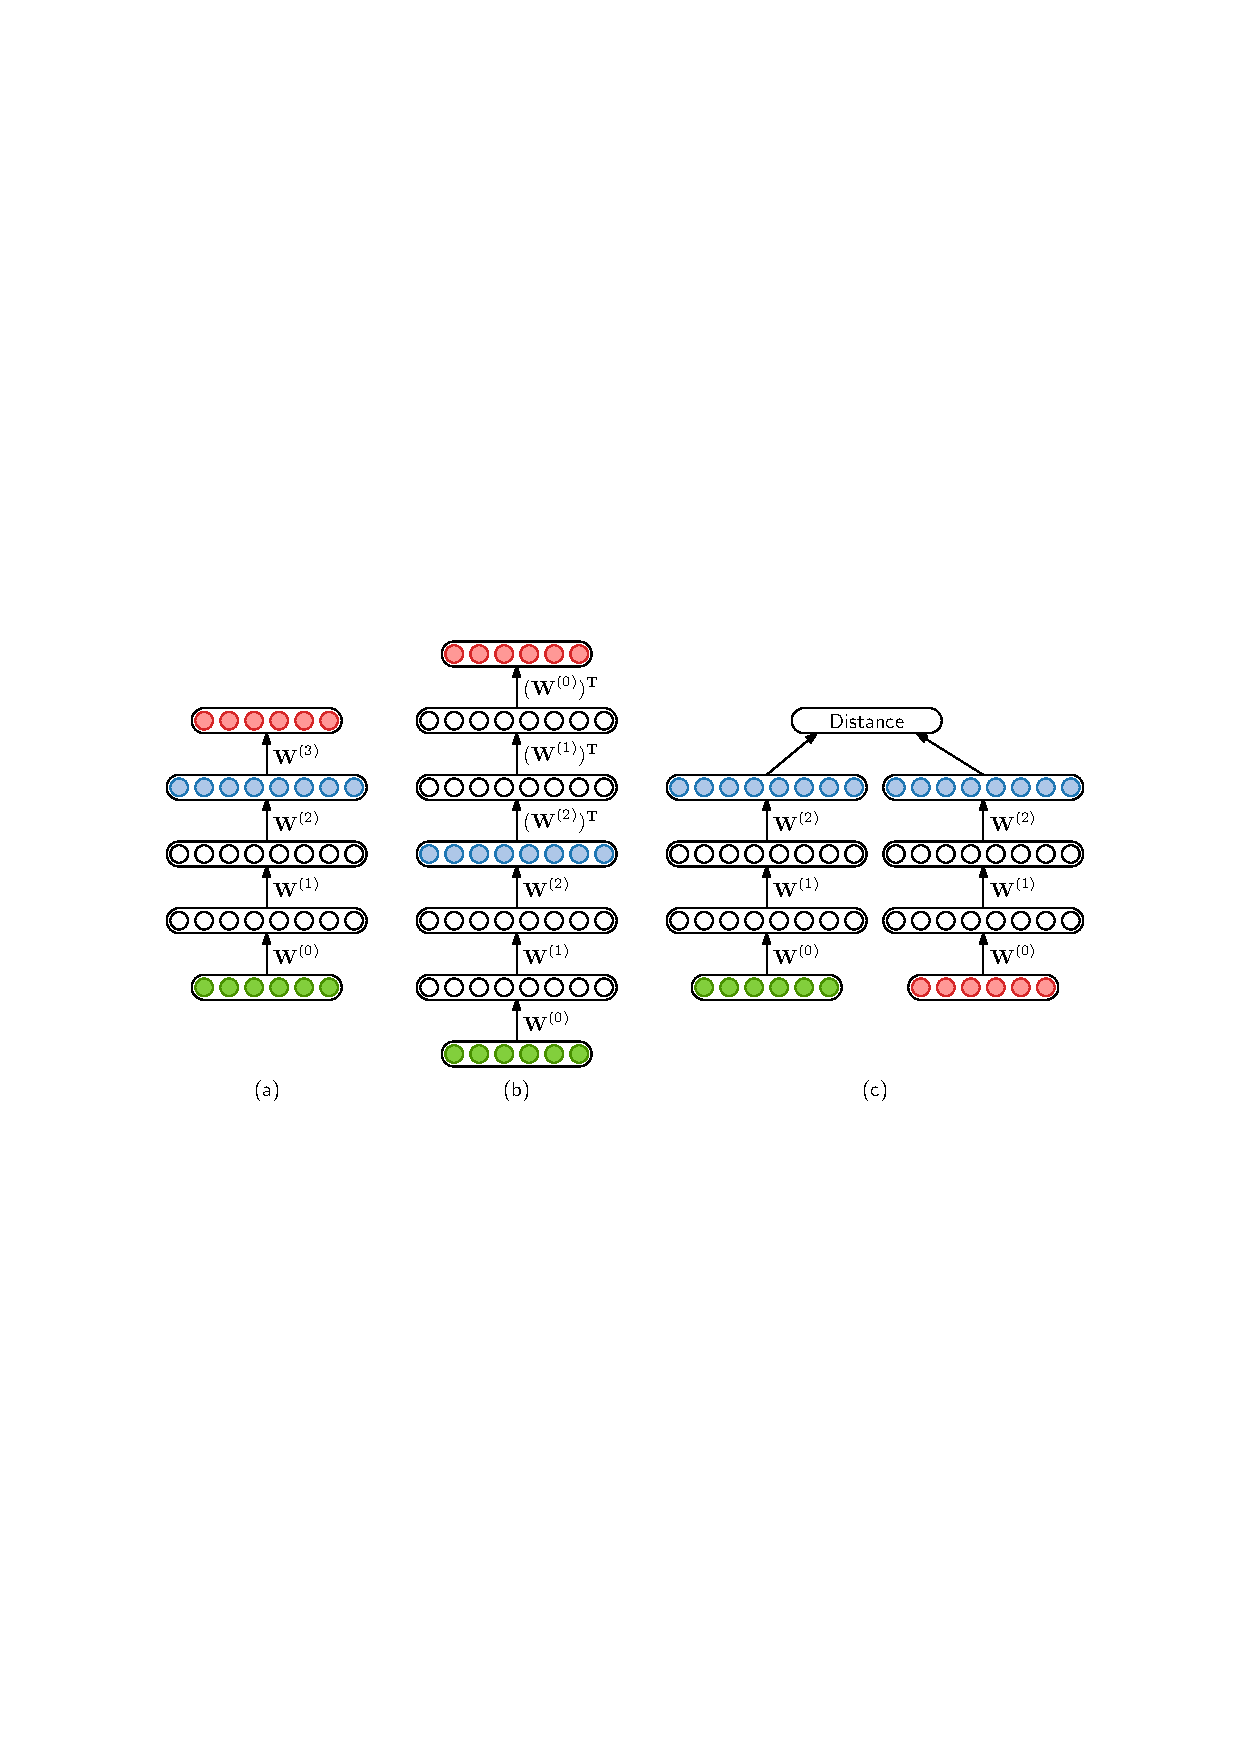
\includegraphics[width=\linewidth]{cae_siamese}
            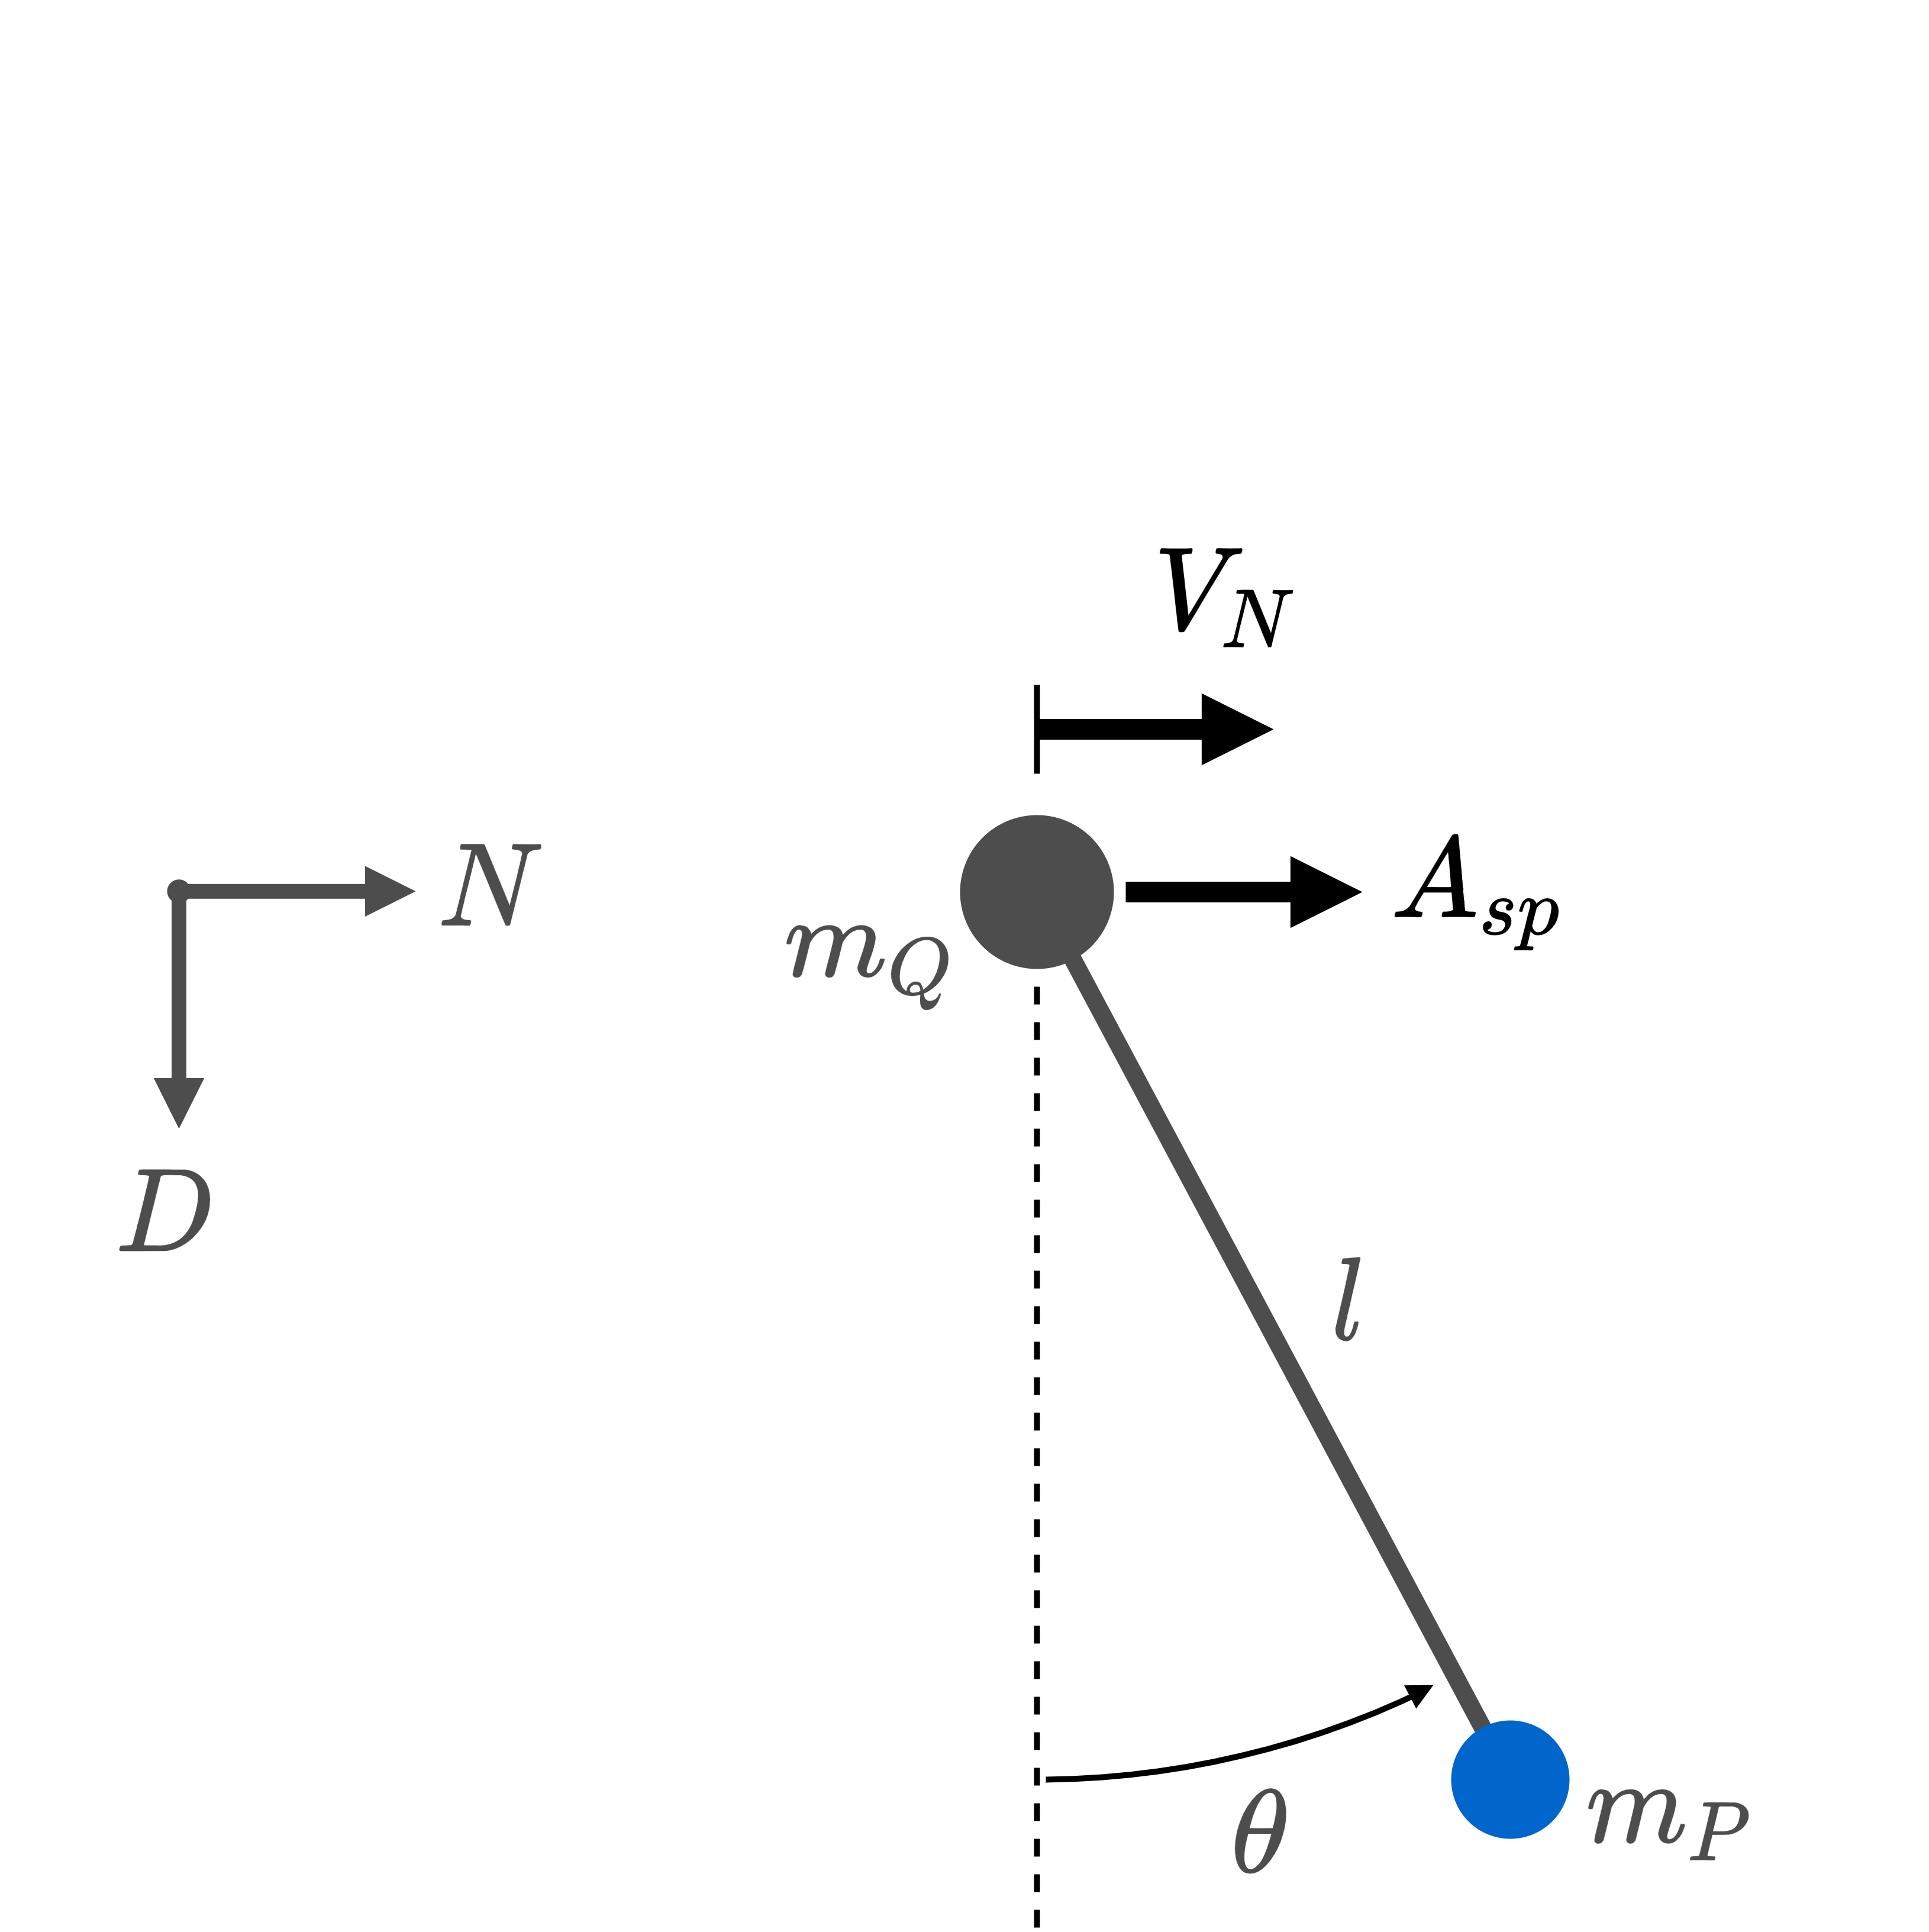
\includegraphics[width=0.5\linewidth]{floating_pend.png}            
            \caption{Floating pendulum model considered for system identification for a North velocity controller}
            \label{fig:floating_pend}
        \end{figure}
    
        \paragraph{Derived model}
        Figure \ref{fig:floating_pend} shows the plant considered for system identification.
        In Chapter~\ref{chap:modelling} the differential equations that describe the motion of this system are derived with Lagrangian mechanics.
        From these equations it is clear that the considered plant is defined by the state vector,
        \begin{equation}
            \bm{x} = \begin{bmatrix}
                V_N & \dot{\theta}
            \end{bmatrix}^T,
        \end{equation}
        and the input vector,
        \begin{equation}
            \bm{u} = \begin{bmatrix}
                A_{N,sp}
            \end{bmatrix},
        \end{equation}
    
        % From this derivation it is clear that the angular velocity of the payload, $\dot{\theta}$, is required to described the system dynamics.
        % However, $\dot{\theta}$ is not measured directly on the considered practical quadrotor setup.
        % Instead, the payload angle, $\theta$, is measured by a potentiometer attached to a ADC on Honeybee as described in Chapter \ref{chap:system_overview}.
        % As expected, this measurement is extremely noisy.
        % \murray{Maybe insert figure to show noise}
        % % Figure \ref{} shows the angle measurement during a practical experiment of the payload while Honeybee is held stationary
        % Numerical differentiation is applied to the noisy $\theta$ signal which results in a very inaccurate estimation of $\dot{\theta}$.
        % Therefore it is desirable to rather use $\theta$ in the system identification process. 

\section{Parameter estimation}
    \subsection{Predetermined linear model}
        The motivation for paramater estimation is to determine unknown parameter values required by the predetermined model.
        This model was derived a prioiri in Section~\ref{sec:linear_model}.
        
    \subsection{Payload mass estimation}
        RLS

    \subsection{Cable length estimation}
        The cable length is estimated from the measurement of natural frequency of the swinging payload.
        As described by
        \cite{bisgaard},
        the natural frequency is given by:
        \begin{equation} \label{eq:nat_freq}
            \omega_n = \sqrt{ \frac{g}{l} \cdot \frac{m_q + m_p}{m_q}}
        \end{equation}
        The natural frequency is measured by performing a FFT on the payload swing angle response after a position step by the quadrotor.
        The dominant frequency identified by the FFT during free swing is the natural frequency of the payload.
        
        \ref{fig:pos_step_angle}
        shows the payload swing angle after the system is stimulated by a position step setpoint.
        As shown in 
        \ref{fig:pos_step_angle}
        the first few seconds of the step response are not used in the FFT.
        This is to minimise the effect of the quadrotor controllers on the swing angle frequency 
        by excluding the transient response in the FFT.

        \ref{fig:fft} 
        shows the resulting amplitude spectrum of the payload swing angle response.
        The dominant frequency is clearly identified as ??.
        Since $m_q$ and $g$ is known, and $m_p$ and $\omega_n$ has been estimated, $l$ can now be determined from
        \ref{eq:nat_freq}.
        In this case the estimated length is ??, compared to the actual length of ??.
        
        Frequency resolution ??
        error for different lengths??
  
\section{Dynamic Mode Decomposition with control}
\label{sec:dmdc}
    
    \paragraph{Intro}        
    DMD is a linear regression technique that can be used to approximate a non-linear dynamical system \cite{Tu2014}.
    It uses temporal measurements of system outputs to reconstruct system dynamics without prior modelling assumptions.
    DMDc is an adaptation of DMD that also accounts for control inputs \cite{Proctor2016c}.
    This section provides an overview of the specific implementation of DMDc used in this paper.        
    Note that this implementation is a slight adaptation of DMDc, and includes time-delay-embedding of multiple observables. 
    \cite{Korda2018b} and \cite{Arbabi2018} use time-delay-embedding in their DMD adaptions in similar ways.

    \paragraph{State space model}
    DMD produces a linear, discrete state-space model of the system dynamics.
    Discrete measurements, $\bm{x}_k$, of the continuous time observable, $\bm{x}(t)$, are used, 
    where $\bm{x}_k = \bm{x}(k T_s)$, and $T_s$ is the sampling time of the model.    
    Delay-coordinates (i.e. $\bm{x}_{k-1}, \bm{x}_{k-2}$, etc.) are also included in the state-space model to
    account for input delay and state delay in the system.
    Input delay refers to the time delay involved with transporting a control signal to a system, 
    whereas state delay refers to time-separated interactions between system variables \cite{Chen1999}.
    Hence, we define an state delay vector as:
    \begin{equation}
        \bm{d}_{k} = 
        \begin{bmatrix}
            \bm{x}_{k-1} & \bm{x}_{k-2} & \cdots & \bm{x}_{k-q}
        \end{bmatrix}^T ,
    \end{equation}
    $\bm{d}_k \in \R^{(n_x)(q)}$ and where $q$ is the number of delay-coordinates used in the model.
    
    \paragraph{}
    The discrete state-space model is therefore defined as:
    \begin{equation} \label{eq:dmd_state_space}
        \bm{x}_{k+1} = \bm{A} \bm{x}_k + \bm{A}_d \bm{d}_k + \bm{B} \bm{u}_k ,
    \end{equation}
    \( \bm{A} \in \R^{n_x \times n_x} \) is the system matrix, 
    \( \bm{A}_1 \in \R^{(q \cdot n_x) \times (q \cdot n_x)} \) is the state delay system matrix and 
    \( \bm{B} \in \R^{n_x \times n_u} \) is the input matrix.
    
    \paragraph{Training data}
    The training data consists of full-state measurements, $\bm{x}_k$, and corresponding inputs, $\bm{u}_k$, 
    taken at regular intervals of $\Delta t = T_s$, during a simulated flight with Cascaded PID control.
    In a practical flight, these time-series measurements need to be saved in memory because it is usd as a single batch by DMD.
    Note that DMD can be applied in a recursive manner as described in \cite{Noack2016}, 
    However this implementation is not considered because memory size will not be a limitation since a companion computer will be used.
    
    \paragraph{Data matrices}
    The training data is collected into the following matrices:
    \begin{align} \label{eq:dmd_matrices}
        \bm{X^\prime} = & \phantom{.} \left [
            \begin{array}{*{5}{@{}M{\mycolwd}@{}}}
                    \bm{x}_{q+2} & \bm{x}_{q+3} & \bm{x}_{q+4} & \cdots & \bm{x}_{w+q+1}
            \end{array}
        \right ] , \nonumber \\
        %
        \bm{X} \phantom{''} = & \phantom{.} \left [
            \begin{array}{*{5}{@{}M{\mycolwd}@{}}}
                \bm{x}_{q+1} & \bm{x}_{q+2} & \bm{x}_{q+3} & \cdots & \bm{x}_{w+q}                      
            \end{array}
        \right ] , \nonumber \\
        % 
        \bm{X}_d \phantom{'} = & \phantom{'} \left [
            \begin{array}{*{5}{@{}M{\mycolwd}@{}}}
                \bm{x}_{q} & \bm{x}_{q+1} & \bm{x}_{q+2} & \cdots & \bm{x}_{w+q-1} \\
                \vdots   & \vdots   & \vdots   & \ddots & \vdots \\
                \bm{x}_2 & \bm{x}_3 & \bm{x}_4 & \cdots & \bm{x}_{w+1} \\
                \bm{x}_1 & \bm{x}_2 & \bm{x}_3 & \cdots & \bm{x}_{w} \\                       
            \end{array}
        \right ] , \nonumber \\
        % 
        \bm{\Upsilon} \phantom{'} = & \phantom{.} \left [
            \begin{array}{*{5}{@{}M{\mycolwd}@{}}}
                    \bm{u}_{q} & \bm{u}_{q+1} & \bm{u}_{q+2} & \cdots & \bm{u}_{w+q-1}
            \end{array}
        \right ] ,
    \end{align}

    where $w$ is the number of columns in the matrices, 
    $\bm{X^\prime}$ is the matrix $\bm{X}$ shifted forward by one time-step, 
    $\bm{X}_d$ is the matrix with delay states, 
    and $\bm{\Upsilon}$ is the matrix of inputs.
    Equation (\ref{eq:dmd_state_space}) can be combined with the matrices in Equation (\ref{eq:dmd_matrices}) to produce:
    \begin{equation}
        \bm{X^\prime} = \bm{A} \bm{X} + \bm{A}_d \bm{X}_d + \bm{B} \bm{\Upsilon} .
    \end{equation}
    Note that the primary objective of DMDc is to determine the best fit model matrices, $\bm{A}$, $\bm{A}_d$ and $\bm{B}$, 
    given the data in $\bm{X^\prime}$, $\bm{X}$, $\bm{X}_d$, and $\bm{\Upsilon}$ \cite{Proctor2016c}.
    In order to group the unknowns into a single matrix, (\ref{eq:dmd_state_space}) is manipulated into the form,
    \begin{equation} \label{eq:G_Omega}
        \bm{X^\prime} =   
        \begin{bmatrix} 
            \bm{A} & \bm{A}_d & \bm{B} 
        \end{bmatrix}
        \begin{bmatrix} 
            \bm{X} \\ \bm{X}_d \\ \bm{\Upsilon} 
        \end{bmatrix} 
        = \bm{G \Omega} ,
    \end{equation} 
    where $\bm{\Omega}$ contains the state and control data, and $\bm{G}$ represents the system and input matrices.
    
    \paragraph{SVD}
    A SVD is performed on $\bm{\Omega}$ resulting in:
    \(
        \bm{\Omega} = \bm{U} \bm{\Sigma} \bm{V}^T
    \).
    Often, only the first $p$ columns of $\bm{U}$ and $\bm{V}$ are required for a good approximation of the dynamics \cite{Brunton2017a}.
    In many cases, the truncated form results in better models than the exact form when noisy measurements are used.
    This is because the effect of measurement noise is mostly captured by the truncated columns of $\bm{U}$ and $\bm{V}$.
    By truncating these columns, the influence of noise in the regression problem is reduced. \murray{explain this better}
    hence the SVD is used in the truncated form: 
    \begin{equation} \label{eq:tilde_svd}
        \bm{\Omega} \approx \Tilde{\bm{U}} \Tilde{\bm{\Sigma}} \Tilde{\bm{V}}^T ,
    \end{equation}
    where $\phantom{.} \Tilde{ } \phantom{.}$ represents rank-$p$ truncation.
    \murray{maybe insert colour pictures showing matrices}        

    \paragraph{}
    By combining (\ref{eq:tilde_svd}) with the over-constrained equality in (\ref{eq:G_Omega}), 
    the least-squared solution, $\bm{G}$, can be found with:
    \begin{equation}
        \bm{G} \approx \bm{X^\prime} \Tilde{\bm{V}} \Tilde{\bm{\Sigma}}^{-1} \Tilde{\bm{U}} .
    \end{equation}
    By reversing \ref{eq:G_Omega}, $\bm{G}$ can now be separated into:
    \(
        \bm{G} = \begin{bmatrix} \bm{A} & \bm{A}_d & \bm{B} \end{bmatrix}.
    \)
    according to the required dimensions of each matrix.
    Thereby, the state-space model approximated by DMDc is complete.
    
\section{Hankel Alternative View Of Koopman}
    
    \murray{q = number of delays, from here up}
    
    \paragraph{}
    HAVOK is a data-driven, regression technique that provides a connection between DMD and Koopman operator theory \cite{Brunton2017a, Champion2019}. 
    We have adapted the standard HAVOK algorithm slightly to account for the effect of control and to extract a discrete, linear model that approximates the behaviour of a controlled dynamical system.
    In this section, a brief overview is provided for this implementation and expansion of \mbox{HAVOK}.
    % 
    \paragraph{}
    The extracted discrete state-space model is defined as:
    \begin{equation} \label{eq:havoc_state_space}
        \bm{a}_{k+1} = \Tilde{\bm{A}} \bm{a}_k + \Tilde{\bm{B}} \bm{u}_k ,
    \end{equation}
    where $\bm{a}_k$ is the state vector previously defined in Section \ref{sec:dmdc}, 
    \( \Tilde{\bm{A}} \in \R^{(q \cdot n_x) \times (q \cdot n_x)} \) is the system matrix, 
    and \( \Tilde{\bm{B}} \in \R^{(q \cdot n_x) \times n_u} \) is the input matrix. 
    Here, $\Tilde{\phantom{a}}$ is used to differentiate these matrices from $\bm{A}$ and $\bm{B}$ used in DMDc.
    % 
    \paragraph{}
    The original HAVOK algorithm, developed by \cite{Brunton2017}, constructs a Hankel matrix from output variables only. 
    In order to incorporate the effect of control, an extended Hankel matrix, $\bm{\Pi}$, is created by appending a matrix of inputs to a Hankel matrix of measurements:
    \begin{equation} \label{eq:pi_hankel}
        \bm{\Pi} = \phantom{.} \left [
            \begin{array}{*{5}{@{}M{\mycolwd}@{}}}
                    \bm{a}_{q} & \bm{a}_{q+1} & \bm{a}_{q+2} & \cdots & \bm{a}_{w+q-1} \\
                    \bm{u}_{q} & \bm{u}_{q+1} & \bm{u}_{q+2} & \cdots & \bm{u}_{w+q-1}
            \end{array}
        \right ] ,
    \end{equation}
    where $w$ is the number of columns in $\bm{\Pi}$.
    A truncated SVD of this Hankel matrix results in following approximation:
    \begin{equation} \label{eq:havok_svd_tilde}
        \bm{\Pi} \approx \Tilde{\bm{U}} \Tilde{\bm{\Sigma}} \Tilde{\bm{V}}^T ,
    \end{equation}
    where $\Tilde{\phantom{a}}$ represents rank-$p$ truncation.
    It is important to note that the model extracted by HAVOK depends on the choice of hyperparameters, $p$ and $q$.
    The number of samples in the training data, $N_{train} = w + q -1$, also influences the accuracy of the model.
    % 
    \paragraph{}
    The columns of $\Tilde{\bm{V}}$ are the most significant principal components of the system dynamics \cite{Kamb2020}.
    This matrix, $\Tilde{\bm{V}}$, can be considered to contain a time-series of the pseudo-state, $\bm{v}$, such that
    \(
        \Tilde{\bm{V}}^T = \begin{bmatrix} 
            \bm{v}_q & \bm{v}_{q+1} & \cdots & \bm{v}_w 
        \end{bmatrix} ,
    \)
    characterises the evolution of the actual dynamics in an eigen-time-delay coordinate system \cite{Brunton2017}.
    % 
    Consider the following discrete, state-space formulation:
    \begin{equation} \label{eq:v_ss}
        \bm{v}_{k+1} = \bm{\Lambda} \bm{v}_k .
    \end{equation}
    Recall that DMDc finds a best fit linear operator that directly maps $\bm{a}_{k}$ to $\bm{a}_{k+1}$.
    Similarly, HAVOK determines the best fit linear operator $\bm{\Lambda}$ that maps the pseudo-state $\bm{v}_k$ to $\bm{v}_{k+1}$.
    So, in order to setup an over-determined equality for (\ref{eq:v_ss}), $\Tilde{\bm{V}}^T$ is divided into two matrices:
    \begin{align} \label{eq:v1v2}
        \bm{V}_1 &= \left [
            \begin{array}{*{5}{@{}M{\mycolwd}@{}}} 
                \bm{v}_{q \phantom{-1}}     & \bm{v}_{q+1} & ... & \bm{v}_{w-1} \\
            \end{array} 
        \right ] , \nonumber \\ 
        \bm{V}_2 &= \left [
            \begin{array}{*{5}{@{}M{\mycolwd}@{}}} 
                \bm{v}_{q+1}     & \bm{v}_{q+2} & ... & \bm{v}_{w \phantom{-1}} \\
            \end{array} 
        \right ] ,
    \end{align} 
    where $\bm{V}_2$ is $\bm{V}_1$ advanced a single step forward in time.
    The matrices from Equation (\ref{eq:v1v2}) are now combined with Equation (\ref{eq:v_ss}) and the best fit $\bm{\Lambda}$ is determined with the Moore-Penrose pseudoinverse:
    \begin{equation} \label{eq:v_dmd}
        \bm{V}_2 = \bm{\Lambda} \bm{V}_1 \phantom{---} \Rightarrow \phantom{---} \bm{\Lambda} \approx \bm{V}_1 \bm{V}_1^{\dagger}
    \end{equation}
    % 
    It can be shown from Equation (\ref{eq:havok_svd_tilde}) that Equation (\ref{eq:v_ss}) is transformed from the eigen-time-delay coordinate system to the original coordinate system as the following:
    \begin{equation} \label{eq:v_ss_a} 
        \begin{bmatrix}
            \bm{a}_{k+1}  \\  \bm{u}_{k+1} 
        \end{bmatrix}
    \phantom{.} = \phantom{.} (\Tilde{\bm{U}} \Tilde{\bm{\Sigma}}) \bm{\Lambda} (\Tilde{\bm{U}}  \Tilde{\bm{\Sigma}})^{\dagger} \phantom{.}
        \begin{bmatrix}
            \bm{a}_{k}  \\  \bm{u}_{k} 
        \end{bmatrix} .
    \end{equation}    
    % 
    This form is used to extract $\Tilde{\bm{A}}$ and $\Tilde{\bm{B}}$ from the matrix,
    \( 
        (\Tilde{\bm{U}} \Tilde{\bm{\Sigma}}) \bm{\Lambda} (\Tilde{\bm{U}}  \Tilde{\bm{\Sigma}})^{\dagger}
    \), in the following way:
    \begin{equation} \label{matrix_decomp}
        \begin{bmatrix}
            \bm{a}_{k+1}  \\  \bm{u}_{k+1} 
        \end{bmatrix}
        \phantom{.} = \phantom{.} 
        \begin{bmatrix}
            \Tilde{\bm{A}} \phantom{.....} \Tilde{\bm{B}} \\
            \textit{(discarded)}
        \end{bmatrix}
        \phantom{.}
        \begin{bmatrix}
            \bm{a}_{k}  \\  \bm{u}_{k} 
        \end{bmatrix}.
    \end{equation}    
    % 
    % This decomposition is illustrated in Fig.~\ref{fig:lambda_decomp}, where blocks represent different groups of entries in the matrix.
    % \begin{figure}[h]
    %     \includegraphics[scale = 0.45]{Lambda_decomp.png}
    %     \centering
    %     \caption{Illustration of the extraction of $\Tilde{\bm{A}}$ and $\Tilde{\bm{B}}$ from (\ref{eq:v_ss_a})}
    %     \label{fig:lambda_decomp}
    % \end{figure}
    % 
    Note that the matrix entries in (\ref{matrix_decomp}) that map $\bm{u}_k$ to $\bm{u}_{k+1}$ are meaningless for our purposes and are discarded.
    Similarly to DMDc, some matrix entries in $\Tilde{\bm{A}}$ and $\Tilde{\bm{B}}$ are known a priori due to the relative positions of delay coordinates. These are forced to 1 or 0 to improve the prediction performance of the model.
    
    \murray{merge these paragraphs}
    Since the state vector, $\bm{a}$, includes delay-coordinates, some matrix entries are known a priori and are independent of the dynamics. 
    For example, the values of $\bm{x}_{k}$ should be mapped from their position in $\bm{a}_k$ to specific indices in $\bm{a}_{k+1}$. 
    Due to the least-squares fitting and coordinate transformation, DMDc will not produce these exact values in $\bm{A}$ and $\bm{B}$. 
    By forcing each of these matrix entries to 1 or 0, the state-prediction performance of the model is improved.




\section{Implementation and results}
    \subsection{Methodology}
        \paragraph{Simulation environment}

        \paragraph{Method overview}
        \murray{Maybe convert this to a flow diagram}

        \begin{enumerate}
            \item Takeoff and hover
            \item Command a series of velocity step inputs with random step sizes and time intervals
            \item Measure and save input and output data
            \item Apply algorithm to data and generate model
        \end{enumerate}

        \paragraph{}

        \paragraph{Steps and intervals}
        For the training period, different velocity step inputs are commanded with varying time intervals between step commands.
        A algorithm schedules these velocity step commands, by assigning random step values and time-intervals within a specified range.
        The velocity range is determined in simulation by iteratively increasing the maximum velocity step 
        to a safe value where the quadrotor and payload system remain in stable flight.
        The maximum time-interval is set to a value that allows the payload swing to reach a steady-state condition.
        This ensures that the identified model includes transient and steady-state dynamics.

        \paragraph{Why velocity steps?}
        Velocity step commands are used in the training period because this 
        Frequency decomposition stimulates the system for a large range of frequencies.

        \paragraph{Testing data}

        \paragraph{Error metric}
        Each state error signal is scaled by the reciprocal of the maximum value of that state variable in the training data.
        % This is to provide a better representative error when taking the mean of state variable errors.
        This is to ensure that a scale difference in the variable types create a bias in the error metric.
        For example, the quadrotor velocity reaches values of \SI{3}{\metre/\second} but the payload swing angle has a maximum of only \SI[]{0.526}{\radian}.
        The velocity prediction error is therefore inherently larger than the payload angle prediction error
        and will bias the error metric towards favouring models with good velocity predictions.
        The proposed scaled error metric ensures that the MAE of each state variable can be compared to each other.
        It also provides an error metric that is better and unbiased representative of the model prediction performance across all state variables. 

    \subsection{Hyperparameters}
        Fixed size of data
        Fixed sample time
        Fixed pendulum params
        Talk about the "front"
        Also about singular values
        For each of the experiments shown in this chapter, a hyperparameters selected tuned to produced

    \subsection{Sample time}
        best hyperparameters.
        
        Fixed size of data.
        Fixed pendulum params.

    \subsection{Size of training data}
        The length of training data used for system identification also affects the quality of the model produced.
        Figure~\ref{fig:MAE_vs_train} plots the prediciton error metric compared to the length of training data used for the different system identification procedures.
        For each length of training data, the hyperparameter combination producing the lowest prediction error was determined and used.
        From Figure~\ref{fig:MAE_vs_train} it is clear that the prediction error of both methods decrease as the amount of training data increases.
        This trend confirms our intuition that as more data is used in the regression problem, 
        the determined model will better approximates the actual dynamics instead of over-fitting to the training data.
        
        \begin{figure}[H]
    \centering
    \begin{tikzpicture}
        \begin{axis}[
            grid = major,
            xlabel = Length of training data,
            ylabel = MAE,
            x unit = \si{\second},
            y unit = \si{\second},
            xmin = 0,     xmax = 250,
            ymin = 0.015, ymax = 0.04,
            legend cell align = left,
            legend pos = north east,
            grid style = dashed,
            legend style = {font = \scriptsize},
            label style = {font = \scriptsize},
            tick label style = {font = \scriptsize},
            width = 0.95\columnwidth,
            height = 0.5\columnwidth,
            % initialize Dark2
            cycle list/Dark2,
            % combine it with 'mark list*':
            cycle multiindex* list = {
                Dark2\nextlist
            }
        ]
        
        \addplot+[mark=none, style=solid, ultra thick] table[x=T_train, y=MAE_mean, col sep=comma] {system_id/csv/dmd_MAE_vs_Ntrain_single_pend_mp0.2_l0.5.mat.csv};
        \addlegendentry{DMD}
        
        % \addplot+[mark=none, style=solid, ultra thick] table[x=t, y=dx_wl, col sep=comma] {plots/load_vs_no_load_step_10.csv};
        % \addlegendentry{With payload}

        \end{axis}
    \end{tikzpicture} 
    
    \caption{Velocity response to a position step input with $m =$~\SI{2}{\kilo\gram}, $l =$~\SI{1}{\meter}.}
    \label{fig:dx_load_vs_no_load}
\end{figure}

        \paragraph{}
        compared

        \paragraph{}
        In Figure~\ref{fig:MAE_vs_train} it can be seen that after approximately \SI{120}{\second} 
        the prediction error does not significantly improve with more training data.
        It practice less training data is desirable because less flight time will be wasted on training a model before the quadrotor can fly with a updated controller.
        Less training data also corresponds to lower memory usage on quadrotor hardware.
        Such a slight improvement in prediction error also has a negligible effect on control performance and is therefore not worth the increased data requirement.
        Therefore, only \SI{120}{\second} of flight data will be used to train system identification models. 
        
        \paragraph{}

        effect on overfitting
        best hyperparameters
        Fixed sample time
        Fixed pendulum params
    
    \subsection{Noise}
        \paragraph{}
        Measurement noise is \murray{Find reference for measurement noise definition}
        This is bad for system identification because the output signals no longer represent the actual process
        hides the actual dynamics of the system under  
        The IMU, barometer, magnetometer and GPS sensors on the practical quadrotor are used for state estimation 
        and all experience measurement noise.
        The EKF performs sensor fusion and smooths out most of the measurement noise to provide a state estimate that is less noisy than raw sensor values.
        
        \paragraph{}
        The potentiometer and ADC which measure the payload angle on the quadrotor alos has quite a lot of measurement noise.
        However, this signal is not smoothed by an onboard EKF.
        Figure~\ref{fig:payload_noise} shows the noisy payload angle measurement for a practical pendulum test while the quadrotor is held stationary.
        For models using $\theta$ in the state vector instead of $\dot{\theta}$, 
        this noisy signal can be smoothed with \murray{matlab smoother}.
        Figure~\ref{fig:payload_noise_smoothed} compares the noisy payload angle measurement to the smoothed signal and actual payload angle for a simulated flight.
        The is applied as band-limited white-noise and the noise power was iteratively adjusted to match that of the practical payload measurements.
        
        % \input{system_id/plots/payload_noise.tex}
        
        % \input{system_id/plots/payload_noise_smoothed.tex}
        
        \paragraph{}
        However, since there is no direct measurement of $\dot{\theta}$, 
        numerical differentiation is performed on the noisy $\theta$ measurement to estimate $\dot{\theta}$. 
        This amplifies the noise and results in inaccurate $\dot{\theta}$ signal.
        Total variation differentiation is implemented to estimate $\dot{\theta}$ from the noisy measurements more accurately. \cite{}
        Figure~\ref{fig:payload_noise_diff} shows
        
        % \input{system_id/plots/payload_noise_diff.tex} // With TVDiff

        Noise also affects model prediction accuracy and the length of training data required for adequate predictions. 
        
        % \input{system_id/plots/MAE_vs_train_noise.tex}

        effect on overfitting
        best hyperparameters
        Fixed sample time
        Fixed pendulum params
    
    \subsection{System parameters}
        Best hyperparameters.
        Fixed size of data.
        Fixed sample time.

    \subsection{Dynamic payload}
        Data-driven vs Parameter estimation

    \subsection{Practical flight data}
    \subsection{HIL}
        \paragraph{Companion computer}
        \paragraph{Software}
        \paragraph{CPU}
        \paragraph{Memory}


\graphicspath{{conclusion/fig/}}

\chapter{Conclusion} \label{chap:conclusion}

    \paragraph
    This thesis considered the design and practical implementation of a stabilising control architecture for a multirotor with an unknown suspended payload.
    A broad scope was considered which includes two different area of research, namely, 
    \begin{itemize}
        \item Data-driven system identification of the unknown payload dynamics 
        \item Optimal swing damping control of the multirotor-payload system
    \end{itemize}
    The content and outcome of this work will be discussed in this chapter.

    \section{Literature study}

        \paragraph
        Existing solutions for stabilised multirotor control with a suspended payload were identified in the literature.
        The literature study showed that research seldomly includes experimental results or algorithm testing on practical hardware, even though this would provide valuable insight.
        It also showed that most studies do not account for uncertainty in the controlled system.
        A thorough study of the literature showed that some solutions account for parameter uncertainty, but very few assume no knowledge of the payload dynamics.
        
        \paragraph
        Furthermore, the few studies that achieved stabilised control despite unknown dynamics, 
        counteracted the payload effect as an unknown disturbance instead of actively controlling the payload state. 
        This places the focus on robustness rather than smooth control of the complete multirotor-payload system. 

        % \paragraph
        % Therefore, this study aimed to design a stabilising control architecture that achieves smooth control of the complete system without prior payload knowledge.
        % Furthermore, it was deemed important to demonstrate the technique using experimental data and practical computational hardware.

        % \paragraph
        % The controller design started with the mathematical derivation of a dynamical model for a multirotor named Honeybee.
        % The dynamical equations of the multirotor-payload system and PX4 controller architecture were implemented in a Simulink\texttrademark~simulation for controller design and testing.
        
        \paragraph
        An \gls{LQR} controller was identified as a popular baseline controller in the literature and was selected as the baseline swing damping controller for this work.
        The specific \gls{LQR} implementation considered in this work is based on a previous study that only considers parameter uncertainty. 
        This \gls{LQR} controller is based on a linearised, predetermined model of the multirotor-payload system.
        The payload mass and cable length are unknown prior to a flight and are estimated with \gls{RLS} and \gls{FFT} estimators respectively.
    
    \section{System identification}  

        \paragraph
        The baseline parameter estimation technique was described and applied to data from \gls{SITL} simulations with Gazebo.
        It was shown that the white-box model which uses the estimated parameters captured the general shape of the system state predictions well.
        The white-box model with parameter estimation technique was also applied to a dynamic payload simulation.
        An elongated payload was suspended from the multirotor and acted as a double pendulum, inducing irregular oscillations in the system.
        For this use case, the resultant white-box model predictions did not represent the general shape of the payload dynamics.

        \paragraph
        \gls{DMDc} and \gls{HAVOKc} were introduced as the data-driven system identification techniques proposed by this work.
        These linear regression techniques each produce a discrete, linear space-space model of the considered dynamics based on input and output data only.
        The conventional \gls{HAVOK} is not designed to be applied to controlled systems.
        However, this algorithm was extended in this work to account for control inputs in a dynamical system and will be referred to as \gls{HAVOKc}.
        The conventional \gls{DMDc} algorithm was altered to include delay-coordinates in a similar way to \gls{HAVOK}.
        Furthermore, the mathematical complexity of these techniques was described in detail.

        \paragraph
        These algorithms were applied to multiple \gls{SITL} simulations for testing.
        Data was generated by tracking a sequence of random velocity step inputs with the standard PID controllers from PX4.
        This data was split into training and testing sets.
        The algorithms could then be trained on the set of training data and could be validated on the unseen testing set.
        The prediction accuracy of each model produced by these techniques was quantified with an \gls{NMAE} error metric.
        This metric is based on multiple model prediction runs from different initial conditions over a specified time horizon.

        \paragraph
        A hyperparameters search showed a Pareto elbow as a function of the number of delay-coordinates, $q$, such that increasing $q$ passed this elbow does not significantly increase the model accuracy, but does increase model complexity.
        Furthermore, the `double-descent' phenomenon was identified when testing with various lengths of training data.
        It was consistently observed in different experiments that increasing the length of training data past a specific point decreases the prediction accuracy.
        This is unintuitive because longer lengths of training data are expected to increase model accuracy by reducing overfitting.
        
        \paragraph
        Both techniques were shown to be robust to measurement noise.
        It was also shown that the techniques consistently produced accurate models with a range of different system parameters.
        The techniques were also tested with the dynamic pendulum and the prediction models accurately captured the irregular oscillations, despite having no prior knowledge of the payload.
        This showed a major improvement compared to the white-box model.
        For the range of different tests the prediction accuracies of \gls{DMDc} and \gls{HAVOKc} models were similar, hence \gls{DMDc} is preferred due to lower computational complexity.

        % \paragraph
        % The uncertainty considered by the baseline method is that the payload mass and cable length are unknown.
        % The control architecture proposed by this work is not based on a predetermined model of the payload dynamics.
        % This method assumes that the dynamical model of the payload is also unknown prior to flight.
    
    \section{Swing damping controllers}  

        \paragraph
        Furthermore, the different controllers were discussed and tested.
        The cascaded PID controller was described and the gains of each control loop were tuned in simulation.
        This simulation environment was verified with practical data from the Honeybee multirotor and was shown to be an accurate representation of the actual system.
        
        \paragraph
        The baseline \gls{LQR} controller was also described and the weights were tuned for the simulated multirotor-payload system.
        The \gls{LQR} was designed based on the white-box model which uses estimated parameters for each different payload.
        The control architecture proposed in this work includes an \gls{MPC} controller which uses a data-driven system identification model for predictive control.
        The \gls{MPC} implementation from the Model Predictive Control Toolbox\texttrademark~in Simulink\texttrademark~was used and the algorithm was described in detail.
        This controller, using data-driven system identification models, was also successfully applied for swing damping control in simulation.

% ?? Velocity step tests

        \paragraph
        Numerous tests were performed to evaluate the combined system identification and control architectures.
        For each test, the system identification stages firstly produced the parameter estimates and identified model for the \gls{LQR} and \gls{MPC} approaches respectively.
        Thereafter, each controller was applied based on those results.
        For a payload with a simple pendulum model, the \gls{LQR} and \gls{MPC} both achieved stabilised control resulting in near swing free motion.
        The controllers showed similar swing damping performances, but the \gls{MPC} produced a faster settling time.
        The control architectures consistently achieved swing damping control with different payload masses and cable lengths, despite parameter uncertainty for the \gls{LQR} approach and no prior payload knowledge for the \gls{MPC} approach.
        Both controllers also showed acceptable disturbance rejection during a constant unknown step input force to the multirotor.

% ?? consistently
% ?? Shown to be adaptive

        \paragraph
        The control approaches were also tested for the dynamic payload case.
        Despite the data-driven model showing a much better prediction accuracy than the white-box model, the \gls{LQR} and \gls{MPC} approached produced similar swing damping performances.
        It was shown that even though the data-driven model is accurate in the domain of the state and input vectors considered in training, the optimised trajectory of the \gls{MPC} goes beyond that domain.
        Hence, the model approximation is inaccurate and the resulting \gls{MPC} control is suboptimal.
        Both controller responses were not as smooth as for the simple pendulum model.
        However, both controllers showed stabilised swing damping control of the system and reduced system oscillations quickly.

        \paragraph
        The controller architectures were also applied to a simulation where a different multirotor mass was used. 
        The \gls{LQR} controller induced undesirable, high-frequency oscillations in the system response due to the model inaccuracy.
        This is because the baseline approach only considers parameter uncertainty in the payload mass and cable length.
        However, the \gls{MPC} approach produced the same swing-free motion shown in previous simulations and clearly outperformed the \gls{LQR} approach.
        The proposed control architecture does not rely on prior knowledge of the system dynamics, therefore the architecture can adapt to unconsidered system changes without redesigning the implementation.

    \section{Practical implementation}  

        \paragraph
        For experimental work, the hardware and software toolchains were described.
        Numerous practical flights were performed with different payload masses, cable lengths, and with a dynamics payload.
        All conclusions made with simulation data for the system identification methods were verified with practical flight data.
        This further validated that the simulation environment is a good representative of the actual system.
        This also showed that \gls{DMDc} produces accurate prediction models with practical levels of wind disturbances and measurement noise.

        \paragraph
        Finally, \gls{HITL} simulations were performed to demonstrate the computationally intensive controller algorithm working with the actual hardware and software toolchain.
        This involved a complex system of different, interconnected software tools.
        The \gls{MPC} algorithm ran as a standalone \gls{ROS} node on the \gls{OBC} and was generated from Simulink\texttrademark~code.
        Tests showed that the OBC was acceptable for the processing requirements of the \gls{MPC} and the algorithm could run at the desired speed.
        It was also shown that the final system produces smooth, swing damping control of the multirotor-payload system as seen in previous simulations.

        \paragraph
        Overall, it was shown that the full data-driven system identification with \gls{MPC} control architecture produces swing damping control of the multirotor-payload system despite having no prior knowledge of the payload dynamics.
        It was demonstrated that this control architecture works for various configurations with different system parameters and even with a dynamic payload.
        Furthermore, it was demonstrated that an accurate data-driven prediction model could be determined from practical flight data with wind disturbances and measurement noise.
        It was also demonstrated that the available hardware fulfils the computational requirements of the proposed algorithms.
        Finally, it is concluded that the proposed control architecture is practically feasible for stabilised control of a multirotor and suspended payload with unknown dynamics.
        
    \section{Recommended future work}
        
        \paragraph
        The current work can be continued to further show the practical feasibility of this approach.
        It can also be extended to improve the control performance or to solve different control problems with the same approach.
        Recommendations for future work include:
        \begin{itemize}
            \item Perform practical flights with the \gls{MPC} to demonstrate the practical performance of the controller.
            \item Perform practical flights with a rigidly attached container with sloshing fluid to demonstrate the adaptability of this approach to unknown dynamics.
            % \item Adding an input shaper to the controller input to further improve the swing damping performance.
            \item Test the current solution using obstacle avoidance trajectories and manoeuvres that require the payload to follow a specific trajectory instead of a simple non-swing reference.
            \item Add a continuous excitation functionality to continue training the system identification model during flight and possibly adapt to time-variant uncertainty. 
            \item Quantify the domain represented by the state and input vectors considered in the training data. 
            This could be used to adjust the input signal during training to cover a larger domain and ultimately train a model that better represents the system dynamics.
            This would hopefully improve the controller performance with unknown dynamical models.
            \item Compare the proposed control architecture to a non-linear \gls{MPC} using a non-linear data-driven model like \gls{SINDy}
        \end{itemize}



% Bibliography
\bibliography{Thesis.bib}

% End matter
\appendix
\chapter{Project Planning Schedule}
\makeatletter\@mkboth{}{Appendix}\makeatother
\label{appen:derivations_bigramseg}

This is an appendix.

\chapter{Outcomes Compliance}
\makeatletter\@mkboth{}{Appendix}\makeatother
\label{appen:derivations_bigramseg}

This is another appendix.

\end{document}

